%% LyX 2.3.4.2 created this file.  For more info, see http://www.lyx.org/.
%% Do not edit unless you really know what you are doing.
\RequirePackage{fixltx2e}
\documentclass[12pt,american]{book}
\usepackage{fontspec}
\setmainfont[Mapping=tex-text,Numbers=OldStyle]{FreeSerif}
\setsansfont[Mapping=tex-text]{FreeSans}
\setmonofont{FreeMono}
\usepackage[paperwidth=6in,paperheight=9in]{geometry}
\geometry{verbose,tmargin=1in,bmargin=1in,lmargin=1in,rmargin=0.75in}
\usepackage{fancyhdr}
\pagestyle{fancy}
\setcounter{secnumdepth}{-1}
\setcounter{tocdepth}{1}
\usepackage{url}
\usepackage[unicode=true,
 bookmarks=true,bookmarksnumbered=true,bookmarksopen=false,
 breaklinks=true,pdfborder={0 0 0},pdfborderstyle={},backref=false,colorlinks=false]
 {hyperref}
\hypersetup{pdftitle={Michael's Second Cherokee Reader},
 pdfauthor={Michael Joyner},
 pdfsubject={Cherokee Language},
 unicode=true,hypertexnames=false}

\makeatletter

%%%%%%%%%%%%%%%%%%%%%%%%%%%%%% LyX specific LaTeX commands.
\XeTeXdashbreakstate 0
\newcommand{\noun}[1]{\textsc{#1}}
\providecommand\textquotedblplain{%
  \bgroup\addfontfeatures{Mapping=}\char34\egroup}
%% Special footnote code from the package 'stblftnt.sty'
%% Author: Robin Fairbairns -- Last revised Dec 13 1996
\let\SF@@footnote\footnote
\def\footnote{\ifx\protect\@typeset@protect
    \expandafter\SF@@footnote
  \else
    \expandafter\SF@gobble@opt
  \fi
}
\expandafter\def\csname SF@gobble@opt \endcsname{\@ifnextchar[%]
  \SF@gobble@twobracket
  \@gobble
}
\edef\SF@gobble@opt{\noexpand\protect
  \expandafter\noexpand\csname SF@gobble@opt \endcsname}
\def\SF@gobble@twobracket[#1]#2{}

\@ifundefined{date}{}{\date{}}
%%%%%%%%%%%%%%%%%%%%%%%%%%%%%% User specified LaTeX commands.
\usepackage{multicol}
\usepackage{wallpaper}

\AtBeginDocument{
  \def\labelitemi{\large\(\bullet\)}
  \def\labelitemii{\large\normalfont\bfseries{--}}
  \def\labelitemiii{\large\(\ast\)}
  \def\labelitemiv{\large\(\cdot\)}
}

\makeatother

\usepackage{polyglossia}
\setdefaultlanguage[variant=american]{english}
\begin{document}
\begin{sloppy}

\frontmatter{}

\pagestyle{empty}

%\ThisCenterWallPaper{.7}{images/front-page-syllabary-sequoyah-40.png}
\title{ᎹᎦᎵ ᏔᎵᏁ ᏣᎳᎩ ᎠᎪᎵᏰᏗ\\
\rule[0.5ex]{1\linewidth}{1pt}\\
Michael’s Second Cherokee Reader}
\author{Michael W S Joyner}

\maketitle
\cleardoublepage{}

~

\clearpage{}

\vspace*{\fill}

ᎹᎦᎵ ᏔᎵᏁ ᏣᎳᎩ ᎠᎪᎵᏰᏗ

Michael’s Second Cherokee Reader

Copyright 2014, Michael Joyner

ISBN: 978-X-XXX-XXXXX-X

This work is licensed under the \noun{Creative Commons Attribution-Share
Alike 3.0 United States License}.

\$Revision: 1.49 \$

\$Date: 2014/09/12 03:29:27 \$ UTC

\cleardoublepage{}

\tableofcontents{}

\cleardoublepage{}

\vspace*{\fill}

\noindent \begin{center}
\includegraphics[width=0.99\columnwidth,height=0.99\paperheight,keepaspectratio]{../Michaels-Cherokee-Reader/artwork/syllabarychart}
\par\end{center}

\vspace*{\fill}

\cleardoublepage{}

\pagestyle{plain}

\mainmatter{}

\include{preface}

\chapter{ᎠᏂᏦᎢ ᏧᎾᏍᏗ ᏏᏆ}

ᏧᏟᎢᎸᏔᏅ ᎠᏂᏦᎢ ᏧᎾᏍᏗ ᏏᏆ ᎨᏎ. ᏧᎬᏩᎶᏗ ᎤᏂᏯᎸᏎ. ᎢᎬᏱ ᏏᏆ ᎠᎴ ᎠᏍᎦᏯ ᏚᎾᏠᏎ. ᎢᎦᏓ ᏂᏕᎦᏛᎥ
ᎧᏁᏍᎦ ᏚᎾᎡ Ꮎ ᎠᏍᎦᏯ ᎠᎴ ᏏᏆ ᎤᏛᏁ:—

“ᎰᏍᏓ ᎠᏍᎦᏯ, ᎢᎦᏓ ᎧᏁᏍᎦ ᏗᏍᎬᏏ ᎦᎵᏦᏕ ᎠᏆᏁᏍᎨᏗ ᎠᏆᏚᎵ.”

ᎢᏳᏍᏗ ᎠᏍᎦᏯ ᏄᏛᏁᎴ ᎠᎴ Ꮎ ᎤᏍᏗ ᏏᏆ ᎤᏤᎵ ᎦᎵᏦᏕ ᎤᏁᏍᎨᎮ ᎬᏗ ᎧᏁᏍᎦ. ᎩᎳᏊ ᏩᎭᏯ ᎤᎷᏤ ᎤᎿ.
ᎦᎶᎯᏍᏗ ᎤᏩᏂᎴ ᎠᎴ ᎤᏛᏁ:—

“ᎤᏍᏗ ᏏᏆ, ᎤᏍᏗ ᏏᏆ, ᏥᏴᎭ!”

Ꮎ ᎤᏍᏗ ᏏᏆ ᎤᏬᎯᎵᏴᏎ:—

“ᎥᏝ! ᎥᏝ! ᏣᏲ ᏩᎭᏯ! ᎬᏚᎢᏍᏗᎮ ᎥᏝ!”

ᎾᎯᏳᏃ ᏩᎭᏯ ᎤᏬᎯᎵᏴᏎ:—

“ᎥᏍᎩᏅᏳᏍᏗ, ᏛᏦᏔᎯ ᎠᎴ ᏛᏦᏔᎯ! ᎾᎯᏳ ᏣᏤᎵ ᎦᎵᏦᏕ ᏓᏲᏥ!”

ᎾᎯᏳᏃ ᎤᏦᏔᎮ ᎠᎴ ᎤᏦᏔᎮ ᎠᎴ ᎦᎵᏦᏕ ᎤᏲᏤ ᏃᏊᎴ ᏩᎭᏯ ᎢᎬᏱ ᏏᏆ ᎤᏩᏯᎡᎾ.

Ꮎ ᏔᎵᏁ ᎤᏍᏗ ᏏᏆ ᎠᎨᏯ ᏚᎾᏠᏎ. ᎢᎦᏓ ᎠᏓ ᏚᏩᏰ ᎠᎴ ᏏᏆ ᎤᏛᏁ:—

“ᎰᏍᏓ ᎠᎨᏯ, ᎢᎦᏓ ᎠᏓ ᏗᏍᎩᎥᏏ ᎦᎵᏦᏕ ᎠᏆᏁᏍᎨᏗ ᎠᏆᏚᎵ.”

ᎢᏳᏍᏗ ᎠᎨᏯ ᏄᏛᏁᎴ ᎠᎴ Ꮎ ᎤᏍᏗ ᏏᏆ ᎤᏤᎵ ᎦᎵᏦᏕ ᎤᏁᏍᎨᎮ. ᎾᎯᏳ ᏩᎭᏯ ᎤᎷᏤ ᎤᎿ ᎠᎴ ᎤᏛᏁ:—

“ᎤᏍᏗ ᏏᏆ, ᎤᏍᏗ ᏏᏆ, ᏥᏴᎭ!”

“ᎥᏝ! ᎥᏝ! ᏣᏲ ᏩᎭᏯ! ᎬᏚᎢᏍᏗᎮ ᎥᏝ!”

“ᎥᏍᎩᏅᏳᏍᏗ, ᏛᏦᏔᎯ! ᏛᏦᏔᎯ! ᎠᎴ ᏣᏤᎵ ᎦᎵᏦᏕ ᏓᏲᏥ ᎢᏳᏍᏗ ᏛᏦᏔᎯ!”

ᎾᎯᏳ ᎤᏦᏔᎮ ᎠᎴ ᎤᏦᏔᎮ ᏃᏊᎴ ᎤᏦᏔᎮ ᎠᎴ ᎤᏦᏔᎮ ᎾᎯᏳ ᎦᎵᏦᏕ ᎤᏲᏤ ᎠᎴ ᏩᎭᏯ ᏔᎵᏁ ᏏᏆ ᎤᏩᏯᎡ.

Ꮎ ᏦᎢᏁ ᎤᏍᏗ ᏏᏆ ᎠᏍᎦᏯ ᏚᎾᏠᏎ. ᎢᎦᏓ ᏅᏯ ᏗᏛᏓᏅ ᏥᏚᎮ. ᎤᏍᏗ ᏏᏆ ᎤᏛᏁ:—

“ᎰᏍᏓ ᎠᏍᎦᏯ, ᎢᎦᏓ ᏅᏯ ᏗᏛᏓᏅ ᏍᎩᎥᏏ ᎢᏳᏍᏗ ᎦᎵᏦᏕ ᎠᏆᏁᏍᎨᏗ ᎠᏆᏚᎵ.”

ᎢᏳᏍᏗ ᎠᏍᎦᏯ ᎤᏍᏗ ᏏᏆ ᏚᏁᎴ ᎢᎦᏓ ᏅᏯ ᏗᏛᏓᏅ ᎠᎴ ᏏᏆ ᎤᏤᎵ ᎦᎵᏦᏕ ᎤᏁᏍᎨᎮ ᎬᏗ ᎥᏍᎩᎾ. ᎾᎯᏳ
ᏩᏯᎭ ᎤᎷᏤ ᎤᎿ ᎢᏳᏍᏗ ᏥᏂᏚᏛᏁᎴ ᎠᎴ ᎤᏛᏁ:—

“ᎤᏍᏗ ᏏᏆ, ᎤᏍᏗ ᏏᏆ, ᏥᏴᎭ!”

“ᎥᏝ! ᎥᏝ! ᏣᏲ ᏩᎭᏯ! ᎬᏚᎢᏍᏗᎮ ᎥᏝ!”

“ᎥᏍᎩᏅᏳᏍᏗ, ᏛᏦᏔᎯ! ᏛᏦᏔᎯ! ᎠᎴ ᏣᏤᎵ ᎦᎵᏦᏕ ᏓᏲᏥ ᎢᏳᏍᏗ ᏛᏦᏔᎯ!”

ᎾᎯᏳ ᎤᏦᏔᎮ ᎠᎴ ᎤᏦᏔᎮ ᎠᏎᏃ ᎥᏝ ᎦᎵᏦᏕ ᏳᏲᏤ ᏍᎩᏅᏳᏍᏗ ᏏᏊ ᎤᏦᏔᎮ ᎠᎴ ᎤᏦᏔᎮ ᎠᏎᏃ Ꮟ ᎥᏝ ᎦᎵᏦᏕ
ᏳᏲᏤ. ᎾᎯᏳ ᎤᏬᎵᏤ ᎥᏍᎩᎾ ᎥᏝ ᎦᎵᏦᏕ ᏱᏛᏲᏥ ᎠᎴ ᎤᏛᏁ:—

“ᎤᏍᏗ ᏏᏆ, ᎾᎿ ᎠᏆᏅᏔ ᎣᏍᏓ ᏕᏈᏌᏂ ᏠᎨᏏ.”

“ᎭᏢ?” ᎤᏛᏁ Ꮎ ᎤᏍᏗ ᏏᏆ.

“Ꭳ, ᎠᎨ ᏥᏍᏚ ᎤᏤᎵ ᏠᎨᏏ, ᎠᎴ ᏑᎾᎴ ᏱᏔᏛᏅᎢᏍᏔᏂ ᎠᎭᏂ ᏓᏥᎷᏥ ᎠᎴ ᎢᎦᏓ ᏙᏓᏂᎩᏎᏏ.”

“ᎰᏩᏊ,” ᎤᏛᏁ Ꮎ ᎤᏍᏗ ᏏᏆ, “ᏓᎦᏛᏅᎢᏍᏔᏂ. ᎯᎳ ᎠᏟᎢᎵ ᎩᏂᏅᏍᏗ ᏣᏚᎵ?”

“Ꭳ, ᏑᏓᎵ ᎢᏳᏩᏂᎸ.”

ᎾᎯᏳᏃ ᎨᏎ Ꮎ ᎤᏍᏗ ᏏᏆ ᎯᏍᎩ ᏑᎾᎴ ᎤᏗᏛᎮ ᎠᎴ ᏕᏈᏌᏂ ᏫᏚᎩᏎᎾ ᎢᎬᏱ ᏩᎭᏯ ᎤᎷᏤ (Ꮲ ᏑᏓᎵ ᏧᎷᏤ)
ᎠᎴ ᏧᏛᏁ:—

“ᎤᏍᏗ ᏏᏆ, ᏣᏛᏅᎢᏍᏔᏁᏍ?”

Ꮎ ᎤᏍᏗ ᏏᏆ ᎤᏛᏁ: “ᎠᏆᏛᏅᎢᏍᏔᏁᏍ? ᎦᏳᎳ ᏫᏓᎩᏎᎾ. ᎤᏔᎾ ᎧᎵ ᏧᎳᏍᎩ! ᎣᏍᏓ ᏓᎦᎵᏍᏓᏴᏂ!”

Ꮎ ᏩᎭᏯ ᎤᎿᎸᏤ ᎠᏎᏃ ᎤᏓᏅᏖᏞ, “Ꮟ ᏓᏥᎶᎾᏍᏔᏂ”, ᎾᎯᏳ ᎤᏛᏁ:—

“ᎤᏍᏗ ᏏᏆ, ᎾᎿ ᎠᏆᏅᏔ ᎣᏍᏓ ᏒᎦᏔ ᏡᎬ.”

“ᎭᏢ?” ᎤᏛᏁ Ꮎ ᏏᏆ.

“ᏌᎶᎵ ᎤᏤᎵ ᏠᎨᏏ,” ᏩᎭᏯ ᎤᏁᏤ, “ᎠᎴ ᎥᏝ ᏱᏓᏍᎩᎶᎾᏍᏔᏂ ᎾᎯᏳ ᎠᎭᏂ ᏓᎦᎷᏥ ᎯᏍᎩ
ᏑᎾᎴ ᎠᎴ ᎢᎦᏓ ᏒᎦᏔ ᏙᏓᏂᎩᏎᏏ.”

ᎢᏳᏍᏗ ᏅᎩ ᏑᎾᎴ Ꮎ ᎤᏍᏗ ᏏᏆ ᎤᏗᏛᎮ ᎢᎬᏱ ᏩᎭᏯ ᎤᎷᎯᏍᏗ ᏧᎩᏍᏗ ᎤᏚᎵᎮ Ꮎ ᏏᏆ ᏍᎩᏅᏳᏍᏗ ᎦᏯᏄᎵ
ᏒᎦᏔ ᏚᎩᏒᏎ ᎠᏎᏃ ᎢᏂᎨᎢ ᎨᏎ ᎠᎴ ᎠᏎ ᏡᎬ ᎤᎸᏍᏗ ᎨᏎ. ᎥᏍᎩᎾ ᎢᏴ ᎡᎳᏗ ᎤᎷᏎ ᏩᎭᏯ ᎦᎷᎨ ᎤᎪᎮ.
ᎤᏍᎦᎴ. ᏩᎭᏯ ᎤᎷᏤ ᎤᏛᏁᏃ:—

“ᎤᏍᏗ ᏏᏆ, ᎦᏙ!?! ᏂᎯᏧ ᏣᎷᏤ ᎢᎬᏱ ᎠᏴ? ᎠᏃᏍᏓᏍ ᏒᎦᏔ?”

“ᎥᎥ, ᎠᏃᏍᏓᏒᎢ,” ᎤᏛᏁ ᎤᏍᏗ ᏏᏆ. “ᎡᎳᏗ ᏌᏊ ᏓᎬᏗᏅᏎᎵ.”

ᎾᎯᏳᏃ ᎢᎾᏒᎢ ᎤᏗᏅᏎ. ᏩᎭᏯ ᎠᎩᏍᎨ Ꮎ ᎤᏍᏗ ᏏᏆ ᏧᏪᏅᏒᎢ ᏗᏜ ᎤᎵᏘᏎ. ᏐᎢ ᎢᎦ Ꮎ ᏩᎭᏯ ᎤᎷᏤ ᎤᏛᏁᏃ:—

“ᎤᏍᏗ ᏏᏆ, ᏛᎾᏓᏟᏌᏂ ᎦᏚᎲ ᏒᎯᏰᏱ ᏗᏜ; ᏫᏖᏅᏏᏍ?”

“Ꭳ, Ꭵ,” ᎤᏛᏁ Ꮎ ᏏᏆ, “ᏫᏓᎨᏅᏏ; ᎯᎳ ᎠᏟᎢᎵ ᏔᏛᏅᎢᏍᏔᏂ?”

“Ꮶ ᎠᏟᎢᎵ,” ᎤᏛᏁ ᏩᎭᏯ. ᎢᏳᏍᏗ ᎤᏍᏗ ᏏᏆ ᎤᏪᏅᏎ ᎢᎬᏱ ᏩᎭᏯ ᎠᎴ ᏗᎦᏚᎲ ᎤᎷᏤ. ᎾᎯᏳ
ᎠᏓᎾᏁᏒᎲᏍᎨ ᎠᎴ ᏒᏙᏂ ᎤᏩᏎ. ᎾᎯᏳ ᏏᏆ ᏩᎭᏯ ᎤᎪᎮ. “Ꭳ! ᎦᏙ ᏓᎦᏛᏁᎵ?” ᎤᏓᏅᏖᏞ. ᎦᏯᏄᎵ
ᏒᏙᏂ ᏧᏣᏁ ᎾᎯᏳᏃ ᎤᏰᎶᎢᏍᏗ ᏒᏙᏂ ᎤᏅᏤ ᎠᎴ ᎡᎳᏗ ᎦᏚᏏ Ꮎ ᏏᏆ ᎠᎴ Ꮎ ᏒᏙᏂ ᎤᏁᏅᏎ ᎠᎾᏗᏆᎸᏕᏲᎮ.
ᏩᎭᏯ ᎤᎪᎮ ᎠᎴ ᎤᏍᎦᎴ. ᎾᎯᏳ ᏧᏪᏅᏒᎢ ᏧᎵᏘᏎ. ᎩᎳᏊ ᎢᏴ ᏏᏆ ᏧᏪᏅᏒᎢ ᎤᏪᏅᏎ Ꮎ ᏩᎭᏯ ᎠᎴ ᎤᏃᎮᏞ
ᎥᏍᎩᎾ ᎡᏆ ᎠᏗᏆᎸᏕᏲᎯ ᎨᏒ ᎠᎴ ᏩᎭᏯ ᎠᏍᎦᎯ ᎨᏎ ᎠᎴ ᎥᏍᎩᎾ ᎤᎵᏘᏎ. ᎾᎯᏳ ᎤᏍᏗ ᏏᏆ ᎤᏛᏁ:—

“Ꭽ! ᎯᏍᎦᎯ! ᎠᏴ ᎬᏍᎦᎸᏍᏓᏅ. ᏒᏙᏂ ᎠᏆᏒ ᎾᎯᏳ ᎬᎪᎲ ᎠᎴ ᏒᏙᏂ ᎠᏆᏣᏅ ᎩᎳᏊ ᎢᏴ ᏒᏙᏂ ᎦᏅᎩ
ᎨᏒ ᎠᎴ ᎠᎦᏐᏍᎬᎢ ᎡᎩ ᎨᏒ. ᎦᏣᎥᏍᎩ ᎨᏒ ᎠᎴ ᏂᎯ ᎠᎩᎶᏒ!”

ᎾᎯᏳᏃ Ꮎ ᏩᎭᏯ ᎤᏔᎾ ᎤᎿᎸᏤ ᎠᎴ ᏏᏆ ᏧᏬᏎᎴ, “ᏣᏲᏒᎢ ᏏᏆ! ᏓᎬᏯᏯᎢ! ᎡᎳᏗ ᎠᎱᏣᏬᎳᏛᎢ ᏓᏥᎸᏏ!”

ᏃᏊ Ꮎ ᏏᏆ ᏓᏈᏌᏂ ᏧᎳᏍᎩ ᏚᏩᏂᏍᏔᏁ ᎤᎿ ᏗᎪᏛᏙᏗ. ᎦᏯᏄᎵ ᏧᎳᏍᎩ ᎤᏍᏚᎢᏎ ᎠᎴ ᏩᎭᏯ ᏧᎳᏍᎩᎢ ᎤᎶᏎ!
ᎦᏯᏄᎵ ᏧᎳᏍᎩ ᎤᏭᏢᏁ ᏩᎭᏯ ᎤᏣᎢ ᎨᏎ. Ꮎ ᎤᏍᏗ ᏏᏆ ᏩᎭᏯ ᎤᏩᏂᏍᏔᏁ ᎠᎴ ᏧᏩᏯᎡ.

\clearpage{}
\begin{center}
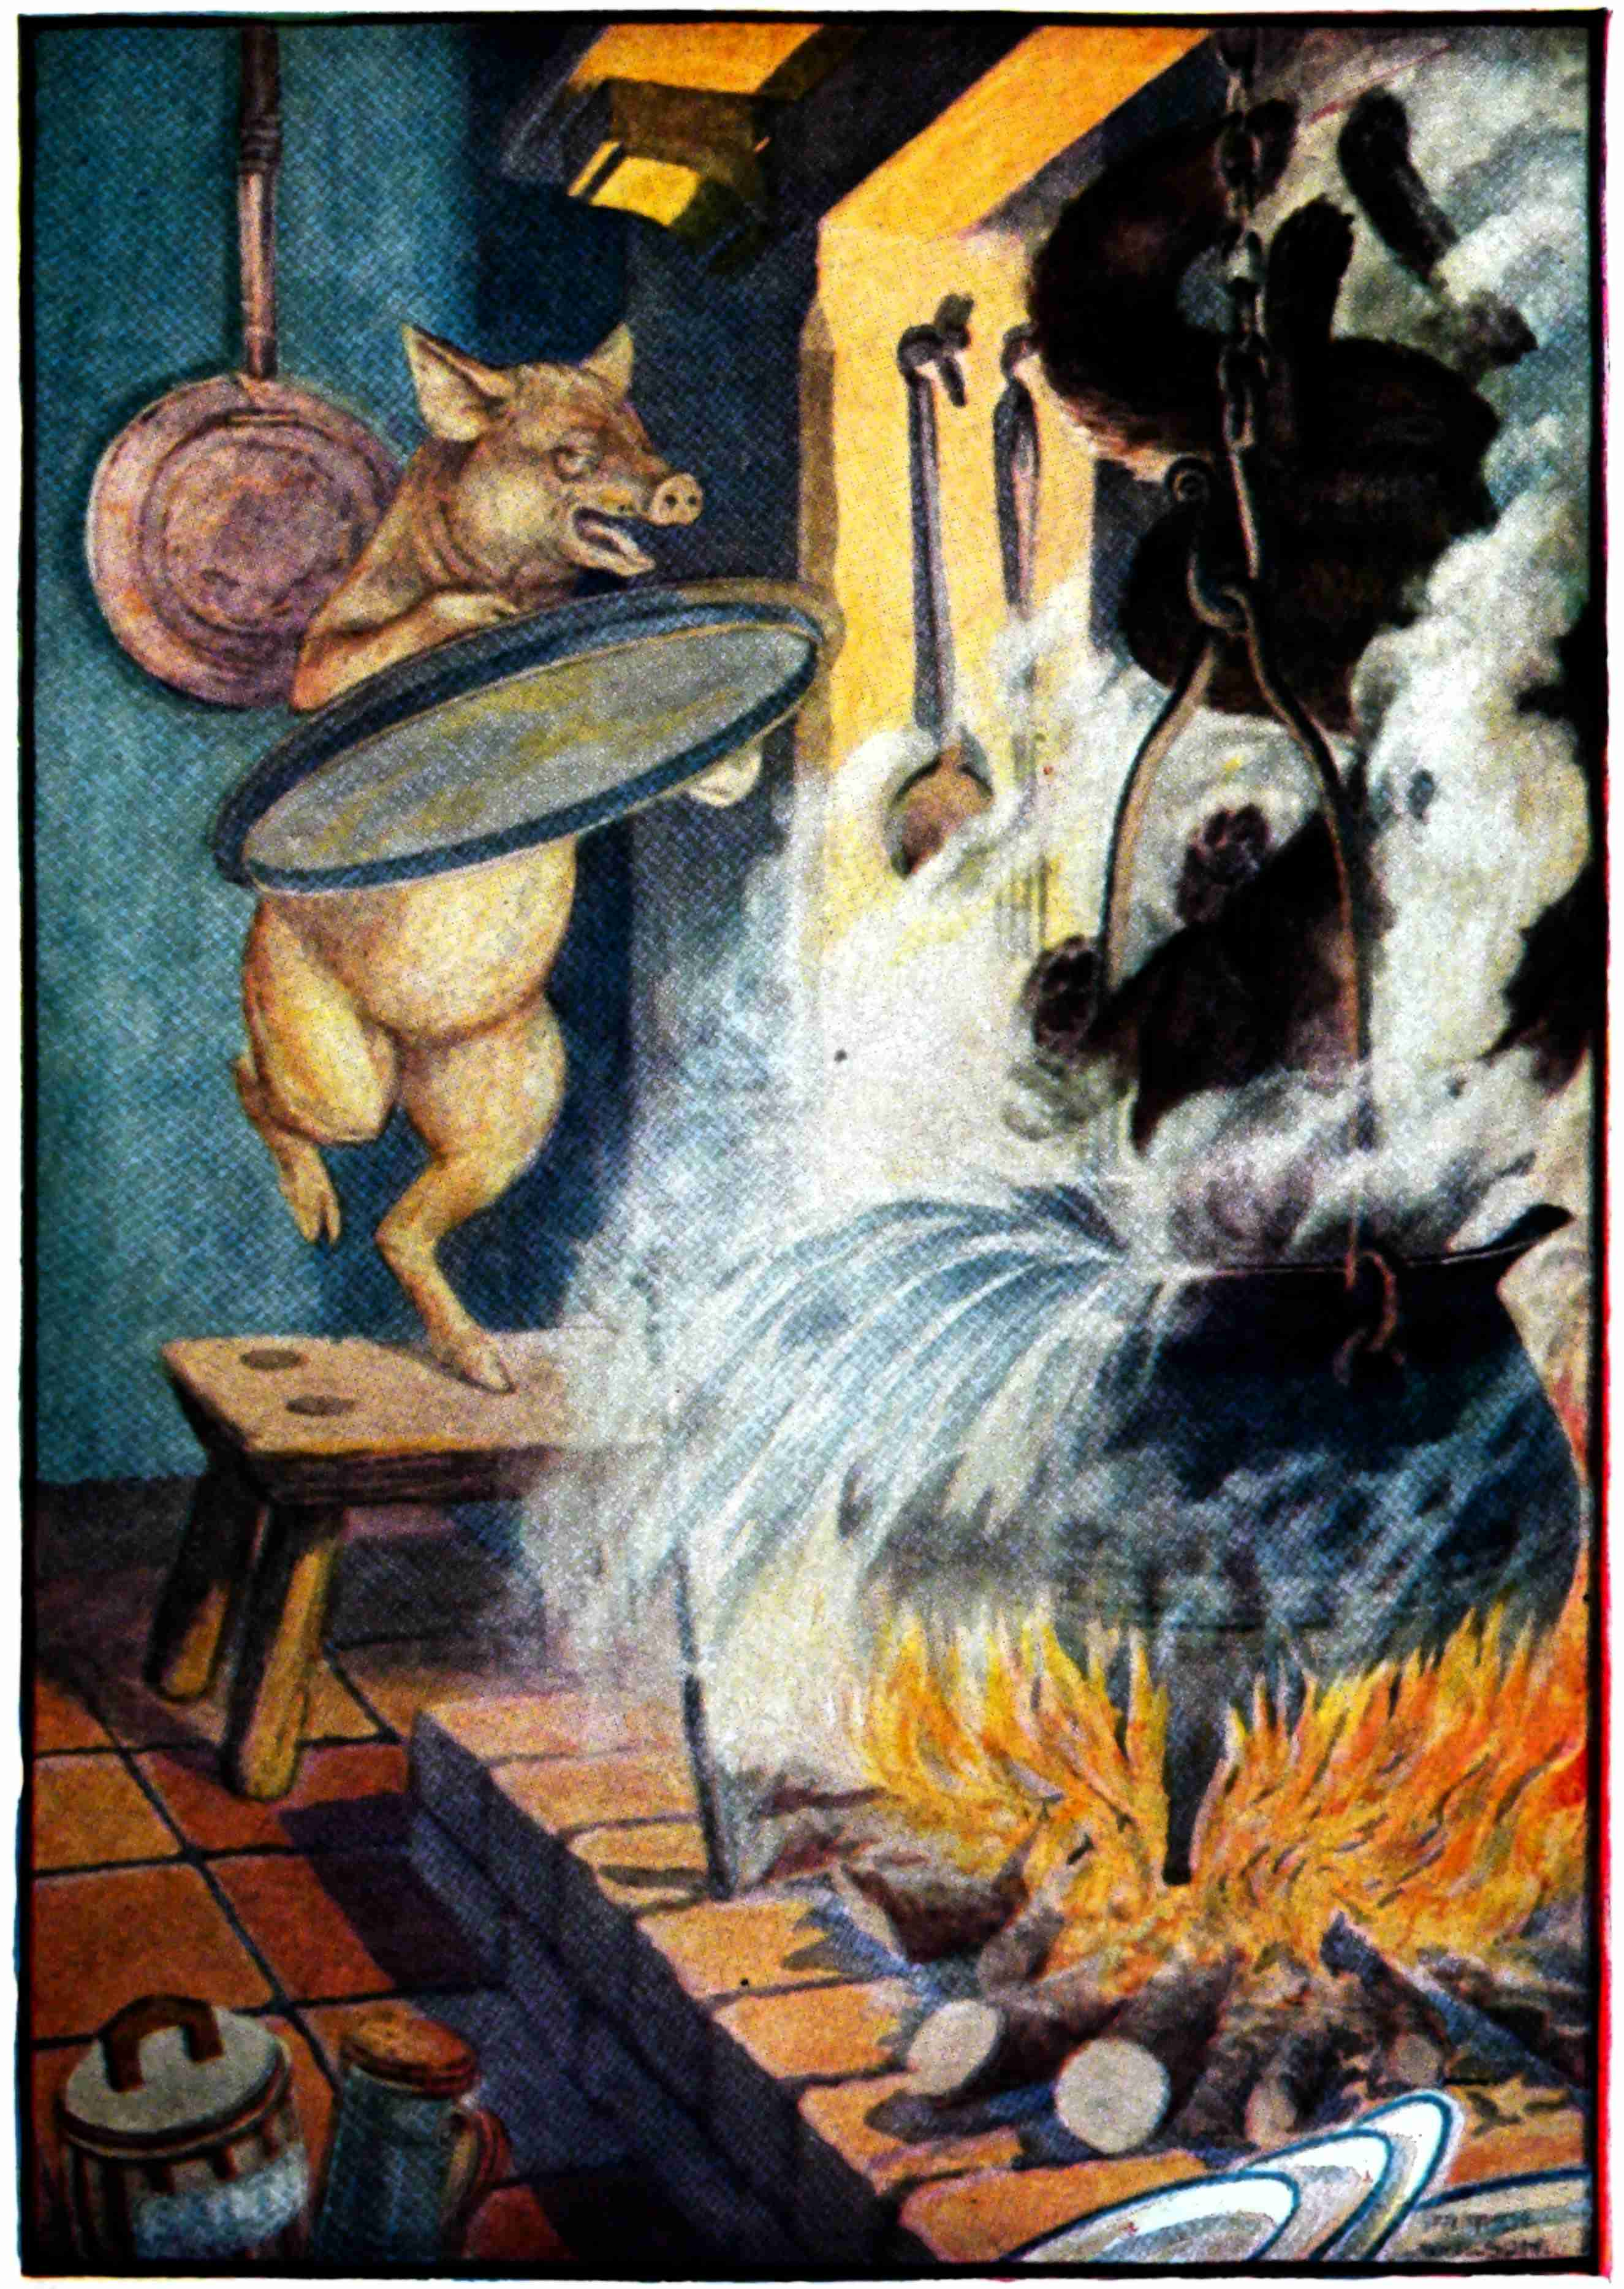
\includegraphics[width=0.99\columnwidth,height=0.99\paperheight,keepaspectratio]{src.jpg/004}
\par\end{center}

\clearpage{}

\chapter{ᏦᎢ ᏲᎾ}

ᏌᏊ ᎢᏳᏩᎦᏗ ᏦᎢ ᏲᎾ ᎨᏎ. ᎢᎾᎨᎢ ᎾᎥ ᎦᎵᏦᏕ ᎠᏁᎯ. ᎢᎬᏱᎢ ᎤᏍᏗᏒ ᏲᎾ, ᏐᎢ ᎠᏰᏟ ᎤᏔᎾ ᏲᎾ,
ᏦᎢᏁ ᎡᏆᏒᎢ ᏲᎾ. 

\include{vocabulary}

%% LyX 2.3.4.2 created this file.  For more info, see http://www.lyx.org/.
%% Do not edit unless you really know what you are doing.
\RequirePackage{fixltx2e}
\documentclass[american]{extbook}
\usepackage{fontspec}
\setmainfont[Mapping=tex-text,Numbers=OldStyle]{FreeSerif}
\setsansfont[Mapping=tex-text]{FreeSans}
\setmonofont{FreeMono}
\usepackage[paperwidth=8.25in,paperheight=11in]{geometry}
\geometry{verbose,tmargin=0.75in,bmargin=0.75in,lmargin=0.85in,rmargin=0.75in}
\pagestyle{plain}
\setcounter{secnumdepth}{-1}
\setcounter{tocdepth}{1}
\setlength{\parskip}{\smallskipamount}
\setlength{\parindent}{0pt}
\PassOptionsToPackage{normalem}{ulem}
\usepackage{ulem}
\usepackage[unicode=true,
 bookmarks=true,bookmarksnumbered=true,bookmarksopen=true,bookmarksopenlevel=0,
 breaklinks=true,pdfborder={0 0 0},pdfborderstyle={},backref=false,colorlinks=false]
 {hyperref}
\hypersetup{
 pdfauthor={Michael Joyner},
 pdfsubject={Cherokee Language},
 unicode=true,plainpages=false,pdfpagelabels,baseurl=http://www.CherokeeLessons.com/,pdfpagelayout=OneColumn}

\makeatletter

%%%%%%%%%%%%%%%%%%%%%%%%%%%%%% LyX specific LaTeX commands.
\XeTeXdashbreakstate 0
\newcommand{\noun}[1]{\textsc{#1}}
\providecommand\textquotedblplain{%
  \bgroup\addfontfeatures{Mapping=}\char34\egroup}
%% Because html converters don't know tabularnewline
\providecommand{\tabularnewline}{\\}

\@ifundefined{date}{}{\date{}}
%%%%%%%%%%%%%%%%%%%%%%%%%%%%%% User specified LaTeX commands.
\usepackage{multicol}
\widowpenalty=10000
\clubpenalty=10000 
\raggedbottom
\usepackage[nottoc]{tocbibind}

\AtBeginDocument{
  \def\labelitemi{\large\(\bullet\)}
  \def\labelitemii{\large\normalfont\bfseries{--}}
  \def\labelitemiii{\large\(\ast\)}
  \def\labelitemiv{\large\(\cdot\)}
}

\makeatother

\usepackage{polyglossia}
\setdefaultlanguage[variant=american]{english}
\begin{document}

\chapter{Grammar}

\emph{Please take note:}
\begin{itemize}
\item The following is from the \textquotedbl\emph{Brief Specimens of
Cherokee Grammatical Forms}\textquotedbl{} as printed in the \textquotedbl\emph{The
Cherokee Messenger (ᏣᎳᎩ ᎠᏥᏅᏏᏛ)}\textquotedbl{} in the years 1844 to
1846.
\item The original text used 'ds' for the soft 'ts' sound. These have been
replaced with 'ts' to be consistent with the entirety of the dictionary.
Additionally “qu” has been replaced with “kw” to be consistent
with the usage of “gw” in the rest of the text.
\item The following description of Cherokee grammar is for 1840's Cherokee
and not today's Cherokee. While most differences between the two are
minor, \emph{there are differences}. The material is very useful when
working with the Cherokee New Testament, the Cherokee translation
of Genesis, the Cherokee translation of Pilgrim's Progress, and so
forth.
\item The English text is also from the 1840's and has not been “modernized”.
It is important to understand that “thee” and “thou” are
used to indicate “you one” and that “ye” and “you”
are used to indicate “you two or more”.
\item Some re-arrangment of text, tables, and minor changes of wording have
happened to facilitate e-book creation.
\end{itemize}
\cleardoublepage{}

\section{\noun{Syllabary}}

\subsection*{\noun{Characters as arranged by the inventor.}}

\textbf{\Huge{}Ꭱ Ꭰ Ꮃ Ꮵ Ꮐ Ꮽ Ꮺ Ꮅ Ꮑ Ꮌ Ꭹ Ᏹ Ꮟ Ꮲ Ꭳ Ꮇ Ꮄ Ꭽ Ꮼ Ꮰ Ꮤ Ᏼ Ꮈ Ꭿ Ꮝ Ᏺ
Ꮁ Ꭺ Ꮷ Ꮍ Ꮞ Ꮠ Ꮯ Ꮘ Ꮗ Ꮜ Ꮖ Ꮓ Ꭷ Ꮸ Ꮢ Ꮒ Ꭶ Ꮩ Ꭸ Ꮣ Ꭼ Ꮻ Ꭲ Ꭴ Ᏸ Ꮂ Ꮫ Ꭻ Ꮶ Ꮙ Ꮔ Ꮎ Ꮆ
Ᏻ Ꮴ Ꮧ Ꮾ Ꮪ Ꮥ Ꮳ Ꭵ Ꮕ Ꮦ Ꮉ Ꮡ Ꮱ Ꭾ Ꮀ Ꮋ Ꮭ Ꮿ Ꮹ Ꮨ Ꮮ Ꮏ Ꮚ Ꮬ Ꮊ Ꮛ.}{\Huge\par}

\subsection*{\noun{Characters systematically arranged with the sounds.}}
\begin{center}
\includegraphics[width=0.98\columnwidth]{\string"artwork/syllabary chart\string".jpg}
\par\end{center}

\subsection*{\noun{Sounds represented by vowels.}}

\begin{tabular}{ll}
a~~~~ & as \emph{a} in \emph{father}, or short as \emph{a} in \emph{rival},\tabularnewline
e~~~~ & as \emph{a} in \emph{hate}, or short as \emph{e} in \emph{met},\tabularnewline
i~~~~ & as \emph{i} in \emph{pique}, or short as \emph{i} in \emph{pin},\tabularnewline
o~~~~ & as \emph{o} in \emph{note}, but approaching to \emph{aw}, in \emph{law},\tabularnewline
u~~~~ & as \emph{oo} in \emph{moon}, or short as \emph{u} in \emph{pull},\tabularnewline
v~~~~ & as \emph{u} in \emph{but}, nasalized.\tabularnewline
\end{tabular}

\subsection*{\noun{Consonant Sounds.}}

g is sounded hard, approaching to k; sometimes before e, i, o, u and
v its sound is k. d has a sound between the English d and t; sometimes
before o, u, and v, its sound is t, when written before l and s the
same analogy prevails.

All other letters as in English.

Syllables beginning with g, except ga, have sometimes the power of
k; syllables written with hl, except tla, sometimes vary to dl; la,
le, li, lo, lu, lv, are sometimes sounded hla, hle, hli, hlo, hlu,
hlv.

\section{\noun{Pronouns}}

The Cherokee language has but two separable personal pronouns, viz.:
First person singular and plural, \emph{A-yv} (ᎠᏴ), “I and we.”
Second person singular and plural, \emph{ni-hi} (ᏂᎯ), “thou and
you.” The third person is indicated by \emph{na} (Ꮎ) or \emph{na-ski}
(ᎾᏍᎩ), “that,” or \emph{hi-ya} (ᎯᏯ) or \emph{hi-a} (ᎯᎠ) “this,”
or by a verb expressing some attribute or condition of the person
spoken of, as:—
\begin{center}
\begin{tabular}{l|l|l}
ᏥᎦᏙᎦ, & tsi-ga-do-ga, & \emph{the one who is standing},\tabularnewline
ᏤᏙᎠ, & tse-do-a, & \emph{the one who is moving about},\tabularnewline
ᏧᏬᎳ, & tsu-wo-hla, & \emph{the one who is sitting down},\tabularnewline
ᏥᎦᏅᎦ, & tsi-ga-nv-ga, & \emph{the one who is lying down},\tabularnewline
ᏨᏓᏯᎢ, & tsv-da-ya-i, & \emph{the one who is coming},\tabularnewline
ᏥᏩᎢ, & tsi-wa-i, & \emph{the one who is going},\tabularnewline
ᏥᏲᎱᏒ, & tsi-yo-hu-sv, & \emph{the one who is dead},\tabularnewline
ᏤᎭ, & tse-ha, & \emph{the one who is living},\tabularnewline
ᏧᏢᎦ, & tsu-tlv-ga, & \emph{the one who is sick},\tabularnewline
\end{tabular}
\par\end{center}

The Cherokee language has a form of personal pronouns, which may be
termed \emph{reflexive}; in which all the distinctions of person are
indicated. This form has the sense of myself, thyself, \&c., as the
following will exhibit.
\begin{flushleft}
\begin{tabular}{l|l|l|l}
\multicolumn{1}{l}{\emph{Singular.}} & \multicolumn{1}{l}{} & \multicolumn{1}{l}{} & \tabularnewline
1st person & ᎠᎬᏒ & a-gwv-sv & \emph{myself,}\tabularnewline
2nd person & ᏨᏒ & tsv-sv & \emph{thyself,}\tabularnewline
3rd person & ᎤᏩᏒ & u-wa-sv & \emph{himself,}\tabularnewline
\end{tabular}
\par\end{flushleft}

\begin{flushleft}
\begin{tabular}{l|l|l|l}
\multicolumn{1}{l}{\emph{Dual.}} & \multicolumn{1}{l}{} & \multicolumn{1}{l}{} & \tabularnewline
1st and 2nd person & ᎩᏅᏒ & gi-nv-sv & \emph{ourselves, (thyself and myself)}\tabularnewline
1st and 3rd person & ᎣᎩᏅᏒ & o-gi-nv-sv & \emph{ourselves, (himself and myself)}\tabularnewline
2nd person & ᏍᏛᏒ & sdv-sv & \emph{yourselves, (two)}\tabularnewline
\end{tabular}
\par\end{flushleft}

\begin{flushleft}
\begin{tabular}{l|l|l|l}
\multicolumn{1}{l}{\emph{Plural.}} & \multicolumn{1}{l}{} & \multicolumn{1}{l}{} & \tabularnewline
1st and 2nd person & ᎢᎬᏒ & i-gv-sv & \emph{ourselves, (yourselves and myself)}\tabularnewline
1st and 3rd person & ᎣᎬᏒ & o-gv-sv & \emph{ourselves, (themselves and myself)}\tabularnewline
2nd person & ᎢᏨᏒ & i-tsv-sv & \emph{yourselves, (three or more)}\tabularnewline
3rd person & ᎤᏅᏒ & u-nv-sv & \emph{themselves}\tabularnewline
\end{tabular}
\par\end{flushleft}

The following table exhibits the possessive pronouns; the object possessed
being singular.
\begin{flushleft}
\begin{tabular}{l|l|l|l}
\multicolumn{1}{l}{\emph{Singular.}} & \multicolumn{1}{l}{} & \multicolumn{1}{l}{} & \tabularnewline
1st person & ᎠᏆᏤᎵ & a-kwa-tse-li & \emph{mine,}\tabularnewline
2nd person & ᏣᏤᎵ & tsa-tse-li & \emph{thine,}\tabularnewline
3rd person & ᎤᏤᎵ & u-tse-li & \emph{his,}\tabularnewline
\end{tabular}
\par\end{flushleft}

\begin{flushleft}
\begin{tabular}{l|l|l|l}
\multicolumn{1}{l}{\emph{Dual.}} & \multicolumn{1}{l}{} & \multicolumn{1}{l}{} & \tabularnewline
1st and 2nd person & ᎩᎾᏤᎵ & gi-na-tse-li & \emph{ours, (mine and thine)}\tabularnewline
1st and 3rd person & ᎣᎩᎾᏤᎵ & o-gi-na-tse-li & \emph{ours, (his and mine)}\tabularnewline
2nd person & ᏍᏓᏤᎵ & sda-tse-li & \emph{yours, (two)}\tabularnewline
\end{tabular}
\par\end{flushleft}

\begin{flushleft}
\begin{tabular}{l|l|l|l}
\multicolumn{1}{l}{\emph{Plural.}} & \multicolumn{1}{l}{} & \multicolumn{1}{l}{} & \tabularnewline
1st and 2nd person & ᎢᎦᏤᎵ & i-ga-tse-li & \emph{ours, (yours and mine)}\tabularnewline
1st and 3rd person & ᎣᎦᏤᎵ & o-ga-tse-li & \emph{ours, (theirs and mine)}\tabularnewline
2nd person & ᎢᏣᏤᎵ & i-tsa-tse-li & \emph{yours, (three or more)}\tabularnewline
3rd person & ᎤᎾᏤᎵ & u-na-tse-li & \emph{theirs.}\tabularnewline
\end{tabular}
\par\end{flushleft}

Two degrees of intensity are denoted by adding \emph{ga} (Ꭶ) and \emph{gaya}
(ᎦᏯ), as \emph{akwatseliga} (ᎠᏆᏤᎵᎦ), “mine” (positively); \emph{akwatseligaya}
(ᎠᏆᏤᎵᎦᏯ), “mine” (really): i.e. “I alone am the real owner.”

When the posession of more than one object is to be denoted, the prefixes
are varied thus:—
\begin{flushleft}
\begin{tabular}{l|l|l|l|l|l}
\multicolumn{1}{l}{\emph{Singular.}} & \multicolumn{1}{l}{} & \multicolumn{1}{l}{} & \multicolumn{1}{l}{} & \multicolumn{1}{l}{} & \tabularnewline
1st person & ᏗᏆ & di-gwa & ᏗᏆᏤᎵ & di-gwa-tse-li & \emph{mine,}\tabularnewline
2nd person & ᏗᏣ & di-tsa & ᏗᏣᏤᎵ & di-tsa-tse-li & \emph{thine,}\tabularnewline
3rd person & Ꮷ & tsu & ᏧᏤᎵ & tsu-tse-li & \emph{his,}\tabularnewline
\end{tabular}
\par\end{flushleft}

\begin{flushleft}
\begin{tabular}{l|l|l|l|l|l}
\multicolumn{1}{l}{\emph{Dual.}} & \multicolumn{1}{l}{} & \multicolumn{1}{l}{} & \multicolumn{1}{l}{} & \multicolumn{1}{l}{} & \tabularnewline
1st and 2nd & ᏗᎩᎾ & di-gi-na & ᏗᎩᎾᏤᎵ & di-gi-na-tse-li & \emph{ours, (mine and thine)}\tabularnewline
1st and 3rd & ᏦᎩᎾ & tso-gi-na & ᏦᎩᎾᏤᎵ & tso-gi-na-tse-li & \emph{ours, (his and mine)}\tabularnewline
2nd person & ᏗᏍᏓ & di-sda & ᏗᏍᏓᏤᎵ & di-sda-tse-li & \emph{yours, (two)}\tabularnewline
\end{tabular}
\par\end{flushleft}

\begin{flushleft}
\begin{tabular}{l|l|l|l|l|l}
\multicolumn{1}{l}{\emph{Plural.}} & \multicolumn{1}{l}{} & \multicolumn{1}{l}{} & \multicolumn{1}{l}{} & \multicolumn{1}{l}{} & \tabularnewline
1st and 2nd & ᏗᎦ & di-ga & ᏗᎦᏤᎵ & di-ga-tse-li & \emph{ours, (yours and mine)}\tabularnewline
1st and 3rd & ᏦᎦ & tso-ga & ᏦᎦᏤᎵ & tso-ga-tse-li & \emph{ours, (theirs and mine)}\tabularnewline
2nd person & ᏗᏣ & di-tsa & ᏗᏣᏤᎵ & di-tsa-tse-li & \emph{yours, (three or more)}\tabularnewline
3rd person & ᏧᎾ & tsu-na & ᏧᎾᏤᎵ & tsu-na-tse-li & \emph{theirs.}\tabularnewline
\end{tabular}
\par\end{flushleft}

In the congugation of verbs the person is indicated by inseparable
prefixes, as:—
\begin{flushleft}
\begin{tabular}{l|l|l|l|l|l}
\multicolumn{1}{l}{\emph{Singular.}} & \multicolumn{1}{l}{} & \multicolumn{1}{l}{} & \multicolumn{1}{l}{} & \multicolumn{1}{l}{} & \tabularnewline
1st person & Ꮵ & tsi & ᏥᏁᎦ & tsi-ne-ga & \emph{I speak,}\tabularnewline
2nd person & Ꭿ & hi & ᎯᏁᎦ & hi-ne-ga & \emph{thou speakest,}\tabularnewline
3rd person & Ꭷ & ka & ᎧᏁᎦ & ka-ne-ga & \emph{he speaks,}\tabularnewline
\end{tabular}
\par\end{flushleft}

\begin{flushleft}
\begin{tabular}{l|l|l|l|l|l}
\multicolumn{1}{l}{\emph{Dual.}} & \multicolumn{1}{l}{} & \multicolumn{1}{l}{} & \multicolumn{1}{l}{} & \multicolumn{1}{l}{} & \tabularnewline
1st and 2nd & ᎢᏂ & i-ni & ᎢᏂᏁᎦ & i-ni-ne-ga & \emph{we (thou and I) speak,}\tabularnewline
1st and 3rd & ᎣᏍᏗ & o-sdi & ᎣᏍᏗᏁᎦ & o-sdi-ne-ga & \emph{we (he and I) speak,}\tabularnewline
2nd person & ᏍᏗ & sdi & ᏍᏗᏁᎦ & sdi-ne-ga & \emph{you (two) speak,}\tabularnewline
\end{tabular}
\par\end{flushleft}

\begin{flushleft}
\begin{tabular}{l|l|l|l|l|l}
\multicolumn{1}{l}{\emph{Plural.}} & \multicolumn{1}{l}{} & \multicolumn{1}{l}{} & \multicolumn{1}{l}{} & \multicolumn{1}{l}{} & \tabularnewline
1st and 2nd & ᎢᏗ & i-di & ᎢᏗᏁᎦ & i-di-ne-ga & \emph{we (you and I) speak,}\tabularnewline
1st and 3rd & ᎣᏥ & o-tsi & ᎣᏥᏁᎦ & o-tsi-ne-ga & \emph{we (they and I) speak,}\tabularnewline
2nd person & ᎢᏥ & i-tsi & ᎢᏥᏁᎦ & i-tsi-ne-ga & \emph{you (three or more) speak,}\tabularnewline
3rd person & ᎠᏂ & a-ni & ᎠᏂᏁᎦ & a-ni-ne-ga & \emph{they speak.}\tabularnewline
\end{tabular}
\par\end{flushleft}

In some tenses the personal prefixes take the following form, as:—
\begin{flushleft}
\begin{tabular}{l|l|l|l|l|l}
\multicolumn{1}{l}{\emph{Singular.}} & \multicolumn{1}{l}{} & \multicolumn{1}{l}{} & \multicolumn{1}{l}{} & \multicolumn{1}{l}{} & \tabularnewline
1st person & Ꮵ & tsi & ᏥᏁᎦ & tsi-ne-ga & \emph{I speak,}\tabularnewline
2nd person & Ꭿ & hi & ᎯᏁᎦ & hi-ne-ga & \emph{thou speakest,}\tabularnewline
3rd person & Ꭷ & ka & ᎧᏁᎦ & ka-ne-ga & \emph{he speaks,}\tabularnewline
\end{tabular}
\par\end{flushleft}

\begin{flushleft}
\begin{tabular}{l|l|l|l|l|l}
\multicolumn{1}{l}{\emph{Dual.}} & \multicolumn{1}{l}{} & \multicolumn{1}{l}{} & \multicolumn{1}{l}{} & \multicolumn{1}{l}{} & \tabularnewline
1st and 2nd & ᎢᏂ & i-ni & ᎢᏂᏁᎦ & i-ni-ne-ga & \emph{we (thou and I) speak,}\tabularnewline
1st and 3rd & ᎣᏍᏗ & o-sdi & ᎣᏍᏗᏁᎦ & o-sdi-ne-ga & \emph{we (he and I) speak,}\tabularnewline
2nd person & ᏍᏗ & sdi & ᏍᏗᏁᎦ & sdi-ne-ga & \emph{you (two) speak,}\tabularnewline
\end{tabular}
\par\end{flushleft}

\begin{flushleft}
\begin{tabular}{l|l|l|l|l|l}
\multicolumn{1}{l}{\emph{Plural.}} & \multicolumn{1}{l}{} & \multicolumn{1}{l}{} & \multicolumn{1}{l}{} & \multicolumn{1}{l}{} & \tabularnewline
1st and 2nd & ᎢᏗ & i-di & ᎢᏗᏁᎦ & i-di-ne-ga & \emph{we (you and I) speak,}\tabularnewline
1st and 3rd & ᎣᏥ & o-tsi & ᎣᏥᏁᎦ & o-tsi-ne-ga & \emph{we (they and I) speak,}\tabularnewline
2nd person & ᎢᏥ & i-tsi & ᎢᏥᏁᎦ & i-tsi-ne-ga & \emph{you (three or more) speak,}\tabularnewline
3rd person & ᎠᏂ & a-ni & ᎠᏂᏁᎦ & a-ni-ne-ga & \emph{they speak.}\tabularnewline
\end{tabular}
\par\end{flushleft}

In some tenses the personal prefixes take the following, as:—
\begin{flushleft}
\begin{tabular}{l|l|l|l|l|l}
\multicolumn{1}{l}{\emph{Singular.}} & \multicolumn{1}{l}{} & \multicolumn{1}{l}{} & \multicolumn{1}{l}{} & \multicolumn{1}{l}{} & \tabularnewline
1st person & ᎠᎩ & a-gi & ᎠᎩᏁᏨ & a-gi-ne-tsv & \emph{I have spoken,}\tabularnewline
2nd person & Ꮳ & tsa & ᏣᏁᏨ & tsa-ne-tsv & \emph{thou hast spoken,}\tabularnewline
3rd person & Ꭴ & u & ᎤᏁᏨ & u-ne-tsv & \emph{he hast spoken,}\tabularnewline
\end{tabular}
\par\end{flushleft}

\begin{flushleft}
\begin{tabular}{l|l|l|l|l|l}
\multicolumn{1}{l}{\emph{Dual.}} & \multicolumn{1}{l}{} & \multicolumn{1}{l}{} & \multicolumn{1}{l}{} & \multicolumn{1}{l}{} & \tabularnewline
1st and 2nd & ᎩᏂ & gi-ni & ᎩᏂᏁᏨ & gi-ni-ne-tsv & \emph{we (thou and I) have spoken,}\tabularnewline
1st and 3rd & ᎣᎩᏂ & o-gi-ni & ᎣᎩᏂᏁᏨ & o-gi-ni-ne-tsv & \emph{we (he and I) have spoken,}\tabularnewline
2nd person & ᏍᏗ & sdi & ᏍᏗᏁᏨ & sdi-ne-tsv & \emph{you (two) have spoken,}\tabularnewline
\end{tabular}
\par\end{flushleft}

\begin{flushleft}
\begin{tabular}{l|l|l|l|l|l}
\multicolumn{1}{l}{\emph{Plural.}} & \multicolumn{1}{l}{} & \multicolumn{1}{l}{} & \multicolumn{1}{l}{} & \multicolumn{1}{l}{} & \tabularnewline
1st and 2nd & ᎢᎩ & i-gi & ᎢᎩᏁᏨ & i-gi-ne-tsv & \emph{we (you and I) have spoken,}\tabularnewline
1st and 3rd & ᎣᎩ & o-gi & ᎣᎩᏁᏨ & o-gi-ne-tsv & \emph{we (they and I) have spoken,}\tabularnewline
2nd person & ᎢᏥ & i-tsi & ᎢᏥᏁᏨ & i-tsi-ne-tsv & \emph{you (three or more) have spoken,}\tabularnewline
3rd person & ᎤᏂ & u-ni & ᎤᏂᏁᏨ & u-ni-ne-tsv & \emph{they have spoken.}\tabularnewline
\end{tabular}
\par\end{flushleft}

\section{\noun{Overview of Verbs}}

The simplest form in which we find being and tense, indicated in Cherokee,
is in the Impersonal Substantive Verb \emph{ge-sv-i} (ᎨᏒᎢ), “being,”
and \emph{i-gi} (ᎢᎩ), “is.”

\subsection{\noun{Indicative Mood}}

\begin{tabular}{l|l|l|l}
Verbal noun, & ᎨᏒᎢ & ge-sv-i & \emph{being}\tabularnewline
Conditional or habitual, & ᎨᏐᎢ & ge-so-i & \emph{is, (usually, habitually, or on certain occasions,)}\tabularnewline
Imperfect - conscious, & ᎨᏒᎩ & ge-sv-gi & \emph{was, (with personal knowlege, or consciousness,)}\tabularnewline
Imperfect - unconscious, & ᎨᏎᎢ & ge-se-i & \emph{was, (without personal knowlege, or consciousness,)}\tabularnewline
Future tense, & ᎨᏎᏍᏗ & ge-se-sdi & \emph{will be.}\tabularnewline
\end{tabular}

The distinctions indicated by the inflections of this verb, are combined
with several of the simple tenses of regular verbs, forming compounds
by which many very minute divisions of time, are marked with great
precision.

The \emph{ge-so-i} (ᎨᏐᎢ) inflection modifies the principal tense,
so, as to indicate the usual, customary or habitual prevalence of
what is affirmed, in quantity, quality or frequency: or under certain
circumstances or conditions.
\begin{quotation}
\noun{Note: }The terms which, in this material, are given to the conjugations,
moods, tenses, and other distinctions, indicated by the inflections
of the Cherokee verb, are only used provisionally; such terms vary
widely in other materials.
\end{quotation}

\subsection{\noun{Conjugations}}

The regular Cherokee verb has nine conjugations, viz:

\begin{tabular}{l|l|l|l}
Radical & ᏥᏁᎦ & tsi-ne-ga & \emph{I speak, or I am speaking.}\tabularnewline
Instrumental & ᏥᏁᎢᏍᏗᎭ & tsi-ne-i-sdi-ha & \emph{I speak with it, \&c.}\tabularnewline
Dative & ᏥᏁᏤᎭ & tsi-ne-tse-ha & \emph{I speak to or for him, \&c.}\tabularnewline
Departing & ᏥᏁᏤᎦ & tsi-ne-tse-ga & \emph{I go (to some place) to speak,}\tabularnewline
Approaching & ᏥᏁᏥᎯᎭ & tsi-ne-tsi-hi-ha & \emph{I come (to some place) to speak,}\tabularnewline
Ambulant & ᏥᏁᏥᏙᎭ & tsi-ne-tsi-do-ha & \emph{I speak about in various places,}\tabularnewline
Frequentative & ᏥᏁᏥᎶᎭ & tsi-ne-tsi-lo-ha & \emph{I speak repeatedly,}\tabularnewline
Perfective or Intensive & ᏥᏁᏥᏏᎭ & tsi-ne-tsi-si-ha & \emph{I speak confirming, or adding force to what has been spoken,}\tabularnewline
Completive or Finishing & ᏥᏁᏦᎲᏍᎦ & tsi-ne-tso-hv-sga & \emph{I speak all, or finish speaking.}\tabularnewline
\end{tabular}

\section{\noun{The Radical Conjugation}}

\subsection{\noun{Indicative Mood}}

\subsubsection{Present Tense and its Modifications.}

\begin{tabular}{l|l|l}
ᎧᏁᎦ & ka-ne-ga & \emph{he is speaking,}\tabularnewline
ᎧᏁᎪᎢ & ka-ne-go-i & \emph{he is peaking habitually, or on certain occasions,}\tabularnewline
ᎧᏁᎬᎩ & ka-ne-gv-gi & \emph{he was speaking with my personal knowledge,}\tabularnewline
ᎧᏁᎨᎢ & ka-ne-ge-i & \emph{he was speaking without my personal knowledge,}\tabularnewline
ᎧᏁᎨᏍᏗ & ka-ne-ge-sdi & \emph{he will be speaking,}\tabularnewline
ᎧᏁᎬᎢ & ka-ne-gv-i & \emph{his speaking, or his word.}\tabularnewline
\end{tabular}

Of these forms, \emph{ka-ne-gv-gi} (ᎧᏁᎬᎩ), indicates the presence
or personal knowledge of the person who relates the fact: \emph{ka-ne-ge-i}
(ᎧᏁᎨᎢ), the absence of personal knowledge.

\subsubsection{The Present Tense, showing the distinctions of person, and the modifications
of tense.}

\emph{Distinctions of Person:}
\begin{flushleft}
\begin{tabular}{l|l|l}
\multicolumn{1}{l}{\emph{Singular.}} & \multicolumn{1}{l}{} & \tabularnewline
1st person & ᏥᏁ- & tsi-ne-\tabularnewline
2nd person & ᎯᏁ- & hi-ne-\tabularnewline
3rd person & ᎧᏁ- & ka-ne-\tabularnewline
\end{tabular}
\par\end{flushleft}

\begin{flushleft}
\begin{tabular}{l|l|l}
\multicolumn{1}{l}{\emph{Dual.}} & \multicolumn{1}{l}{} & \tabularnewline
1st and 2nd & ᎢᏂᏁ- & i-ni-ne-\tabularnewline
1st and 3rd & ᎣᏍᏗᏁ- & o-sdi-ne-\tabularnewline
2nd person & ᏍᏗᏁ- & sdi-ne-\tabularnewline
\end{tabular}
\par\end{flushleft}

\begin{flushleft}
\begin{tabular}{l|l|l}
\multicolumn{1}{l}{\emph{Plural.}} & \multicolumn{1}{l}{} & \tabularnewline
1st and 2nd & ᎢᏗᏁ- & i-di-ne-\tabularnewline
1st and 3rd & ᎣᏥᏁ- & o-tsi-ne-\tabularnewline
2nd person & ᎢᏥᏁ- & i-tsi-ne-\tabularnewline
3rd person & ᎠᏂᏁ- & a-ni-ne-\tabularnewline
\end{tabular}
\par\end{flushleft}

\emph{Modifications of Tense:}
\begin{flushleft}
\begin{tabular}{l|l|l}
-Ꭶ & -ga & \emph{I am, thou art, \&c. speaking.}\tabularnewline
-ᎪᎢ & -go-i & \emph{I am, \&c. speaking habitually or on certain occasions.}\tabularnewline
-ᎬᎩ & -gv-gi & \emph{I \&c. was speaking, with my personal knowledge.}\tabularnewline
-ᎨᎢ & -ge-i & \emph{I \&c. was speaking, without my personal knowledge.}\tabularnewline
-ᎨᏍᏗ & -ge-sdi & \emph{I \&c. will be speaking.}\tabularnewline
-ᎬᎢ & -gv-i & \emph{My, thy, his, \&c. speaking, or word.}\tabularnewline
\end{tabular}
\par\end{flushleft}

By connecting each of these terminations with each of the persons
of the verb, all the modications of this tense will be expressed in
each person, thus, \emph{tsi-ne-ga} (ᏥᏁᎦ), “I am speaking,”
\emph{hi-ne-ga} (ᎯᏁᎦ), “thou art speaking,” \&c.

If the English affixed to each modification of this tense, varied
to suit the person, be affixed to the verb, with the corresponding
termination as in the tables, all the variations of person and tense
will be expressed. This remark is applicable to the other tenses which
admit of similar variations.

\subsubsection{The Immediate Past Tense.}
\begin{flushleft}
\begin{tabular}{l|l|l|l}
\multicolumn{1}{l}{\emph{Singular.}} & \multicolumn{1}{l}{} & \multicolumn{1}{l}{} & \tabularnewline
1st person & ᎥᏥᏁᎩ & v-tsi-ne-gi & \emph{I have just spoken,}\tabularnewline
2nd person & ᎥᎯᏁᎩ & v-hi-ne-gi & \emph{thou hast just spoken,}\tabularnewline
3rd person & ᎥᎧᏁᎩ & v-ka-ne-gi & \emph{he hast just spoken,}\tabularnewline
\end{tabular}
\par\end{flushleft}

\begin{flushleft}
\begin{tabular}{l|l|l|l}
\multicolumn{1}{l}{\emph{Dual.}} & \multicolumn{1}{l}{} & \multicolumn{1}{l}{} & \tabularnewline
1st and 2nd & ᎥᏂᏁᎩ & v-ni-ne-gi & \emph{we (thou and I) have just spoken,}\tabularnewline
1st and 3rd & ᎣᏍᏗᏁᎩ & o-sdi-ne-gi & \emph{we (he and I) have just spoken,}\tabularnewline
2nd person & ᎥᏍᏗᏁᎩ & v-sdi-ne-gi & \emph{you (two) have just spoken,}\tabularnewline
\end{tabular}
\par\end{flushleft}

\begin{flushleft}
\begin{tabular}{l|l|l|l}
\multicolumn{1}{l}{\emph{Plural.}} & \multicolumn{1}{l}{} & \multicolumn{1}{l}{} & \tabularnewline
1st and 2nd & ᎥᏗᏁᎩ & v-di-ne-gi & \emph{we (you and I) have just spoken,}\tabularnewline
1st and 3rd & ᎣᏥᏁᎩ & o-tsi-ne-gi & \emph{we (they and I) have just spoken,}\tabularnewline
2nd person & ᎥᏥᏁᎩ & v-tsi-ne-gi & \emph{you (three or more) have just spoken,}\tabularnewline
3rd person & ᎥᎠᏂᏁᎩ & v-an-ni-ne-gi & \emph{they have just spoken.}\tabularnewline
\end{tabular}
\par\end{flushleft}

The Immediate Past Tense does not admit of being modified like the
present, perfect and future tenses.

\subsubsection{Modifications of the Perfect Tense.}
\begin{flushleft}
\begin{tabular}{l|l|l|l}
Simple Perfect & ᎤᏁᏨ & u-ne-tsv & \emph{he has spoken.}\tabularnewline
Conditional Perfect & ᎤᏁᏦᎢ & u-ne-tso-i & \emph{he has spoken, (whenever certain circumstances have taken place.)}\tabularnewline
Imperfect of the Perfect & ᎤᏁᏨᎩ & u-ne-tsv-gi & \emph{he spoke, with my personal knowledge.}\tabularnewline
Imperfect of the Perfect & ᎤᏁᏤᎢ & u-ne-tse-i & \emph{he spoke, without my personal knowledge.}\tabularnewline
Future of the Perfect & ᎤᏁᏤᏍᏗ & u-ne-tse-sdi & \emph{he will have spoken.}\tabularnewline
Verbal Noun & ᎤᏁᏨᎢ & u-ne-tsv-i & \emph{his having spoken, or his word (already spoken.)}\tabularnewline
\end{tabular}
\par\end{flushleft}

\subsubsection{The Perfect Tense, exhibiting the distinctions of person and modifications
of tense.}

\emph{Distinctions of Person:}
\begin{flushleft}
\begin{tabular}{l|l|l}
\multicolumn{1}{l}{\emph{Singular.}} & \multicolumn{1}{l}{} & \tabularnewline
1st person & ᎠᎩᏁ- & a-gi-ne-\tabularnewline
2nd person & ᏣᏁ- & tsa-ne-\tabularnewline
3rd person & ᎤᏁ- & u-ne-\tabularnewline
\end{tabular}
\par\end{flushleft}

\begin{flushleft}
\begin{tabular}{l|l|l}
\multicolumn{1}{l}{\emph{Dual.}} & \multicolumn{1}{l}{} & \tabularnewline
1st and 2nd & ᎩᏂᏁ- & gi-ni-ne-\tabularnewline
1st and 3rd & ᎣᎩᏂᏁ- & o-gi-ni-ne-\tabularnewline
2nd person & ᏍᏗᏁ- & sdi-ne-\tabularnewline
\end{tabular}
\par\end{flushleft}

\begin{flushleft}
\begin{tabular}{l|l|l}
\multicolumn{1}{l}{\emph{Plural.}} & \multicolumn{1}{l}{} & \tabularnewline
1st and 2nd & ᎢᎩᏁ- & i-gi-ne-\tabularnewline
1st and 3rd & ᎣᎩᏁ- & o-gi-ne-\tabularnewline
2nd person & ᎢᏥᏁ- & i-tsi-ne-\tabularnewline
3rd person & ᎤᏂᏁ- & u-ni-ne-\tabularnewline
\end{tabular}
\par\end{flushleft}

\emph{Modifications of Tense:}
\begin{flushleft}
\begin{tabular}{l|l|l}
-Ꮸ & -tsv & The Perfect Tense.\tabularnewline
-ᏦᎢ & -tso-i & The Conditional Perfect.\tabularnewline
-ᏨᎩ & -tsv-gi & Imperfect of the Perfect. \emph{(With my personal knowledge.)}\tabularnewline
-ᏤᎢ & -tse-i & Imperfect of the Perfect. \emph{(Without my personal knowledge.)}\tabularnewline
-ᏤᏍᏗ & -tse-sdi & Future Perfect.\tabularnewline
-ᏨᎢ & -tsv-i & Verbal Noun.\tabularnewline
\end{tabular}
\par\end{flushleft}

If each of these terminations be connected with each person of the
verb, as in the present tense, all the modifications of the tense
will be expressed, in each person.

\subsubsection{Future Tense, shewing the distinctions of person.}
\begin{flushleft}
\begin{tabular}{l|l|l|l}
\multicolumn{1}{l}{\emph{Singular.}} & \multicolumn{1}{l}{} & \multicolumn{1}{l}{} & \tabularnewline
1st person & ᏓᏥᏁᏥ & da-tsi-ne-tsi & \emph{I will speak,}\tabularnewline
2nd person & ᏘᏁᏥ & ti-ne-tsi & \emph{thou wilt speak,}\tabularnewline
3rd person & ᏓᎧᏁᏥ & da-ka-ne-tsi & \emph{he will speak,}\tabularnewline
\end{tabular}
\par\end{flushleft}

\begin{flushleft}
\begin{tabular}{l|l|l|l}
\multicolumn{1}{l}{\emph{Dual.}} & \multicolumn{1}{l}{} & \multicolumn{1}{l}{} & \tabularnewline
1st and 2nd & ᏓᏂᏁᏥ & da-ni-ne-tsi & \emph{we (thou and I) will speak,}\tabularnewline
1st and 3rd & ᏓᏲᏍᏗᏁᏥ & da-yo-sdi-ne-tsi & \emph{we (he and I) will speak,}\tabularnewline
2nd person & ᏓᏍᏗᏁᏥ & da-sdi-ne-tsi & \emph{you (two) will speak,}\tabularnewline
\end{tabular}
\par\end{flushleft}

\begin{flushleft}
\begin{tabular}{l|l|l|l}
\multicolumn{1}{l}{\emph{Plural.}} & \multicolumn{1}{l}{} & \multicolumn{1}{l}{} & \tabularnewline
1st and 2nd & ᏓᏗᏁᏥ & da-di-ne-tsi & \emph{we (you and I) will speak,}\tabularnewline
1st and 3rd & ᏓᏲᏥᏁᏥ & da-yo-tsi-ne & \emph{we (they and I) will speak,}\tabularnewline
2nd person & ᏓᏥᏁᏥ & da-tsi-ne-tsi & \emph{you (three or more) will speak,}\tabularnewline
3rd person & ᏛᏂᏁᏥ & da-ni-ne-tsi & \emph{they will speak.}\tabularnewline
\end{tabular}
\par\end{flushleft}

\subsubsection{Imperfect of the Future Tense}

\emph{(with my personal knowledge)}
\begin{flushleft}
\begin{tabular}{l|l|l|l}
\multicolumn{1}{l}{\emph{Singular.}} & \multicolumn{1}{l}{} & \multicolumn{1}{l}{} & \tabularnewline
1st person & ᏓᏥᏁᏥᏒᎩ & da-tsi-ne-tsi-sv-gi & \emph{I did will or intend to speak.}\tabularnewline
2nd person & ᏘᏁᏥᏒᎩ & ti-ne-tsi-sv-gi & \emph{thou didst will or intend to speak.}\tabularnewline
3rd person & ᏓᎧᏁᏥᏒᎩ & da-ka-ne-tsi-sv-gi & \emph{he did will or intend to speak.}\tabularnewline
\end{tabular}
\par\end{flushleft}

\begin{flushleft}
\begin{tabular}{l|l|l|l}
\multicolumn{1}{l}{\emph{Dual.}} & \multicolumn{1}{l}{} & \multicolumn{1}{l}{} & \tabularnewline
1st and 2nd & ᏓᏂᏁᏥᏒᎩ & da-ni-ne-tsi-sv-gi & \emph{we (thou and I) did will or intend to speak.}\tabularnewline
1st and 3rd & ᏓᏲᏍᏗᏁᏥᏒᎩ & da-yo-sdi-ne-tsi-sv-gi & \emph{we (he and I) did will or intend to speak.}\tabularnewline
2nd person & ᏓᏍᏗᏁᏥᏒᎩ & da-sdi-ne-tsi-sv-gi & \emph{you (two) did will or intend to speak.}\tabularnewline
\end{tabular}
\par\end{flushleft}

\begin{flushleft}
\begin{tabular}{l|l|l|l}
\multicolumn{1}{l}{\emph{Plural.}} & \multicolumn{1}{l}{} & \multicolumn{1}{l}{} & \tabularnewline
1st and 2nd & ᏓᏗᏁᏥᏒᎩ & da-di-ne-tsi-sv-gi & \emph{we (you and I) did will or intend to speak.}\tabularnewline
1st and 3rd & ᏓᏲᏥᏁᏥᏒᎩ & da-yo-tsi-ne-tsi-sv-gi & \emph{we (they and I) did will or intend to speak.}\tabularnewline
2nd person & ᏓᏥᏁᏥᏒᎩ & da-tsi-ne-tsi-sv-gi & \emph{you (three or more) did will or intend to speak.}\tabularnewline
3rd person & ᏓᏂᏁᏥᏒᎩ & da-ni-ne-tsi-sv-gi & \emph{they did will or intend to speak.}\tabularnewline
\end{tabular}
\par\end{flushleft}

\emph{Distinctions of Person:}
\begin{flushleft}
\begin{tabular}{l|l|l}
\multicolumn{1}{l}{\emph{Singular.}} & \multicolumn{1}{l}{} & \tabularnewline
1st person & ᏗᏥᏁᏥ- & di-tsi-ne-tsi\tabularnewline
2nd person & ᏘᏁᏥ- & ti-ne-tsi\tabularnewline
3rd person & ᏗᎧᏁᏥ- & di-ka-ne-tsi\tabularnewline
\end{tabular}
\par\end{flushleft}

\begin{flushleft}
\begin{tabular}{l|l|l}
\multicolumn{1}{l}{\emph{Dual.}} & \multicolumn{1}{l}{} & \tabularnewline
1st and 2nd & ᏗᏂᏁᏥ- & di-ni-ne-tsi\tabularnewline
1st and 3rd & ᏗᏲᏍᏗᏁᏥ- & di-yo-sdi-ne-tsi\tabularnewline
2nd person & ᏗᏍᏗᏁᏥ- & di-sdi-ne-tsi\tabularnewline
\end{tabular}
\par\end{flushleft}

\begin{flushleft}
\begin{tabular}{l|l|l}
\multicolumn{1}{l}{\emph{Plural.}} & \multicolumn{1}{l}{} & \tabularnewline
1st and 2nd & ᏗᏗᏁᏥ- & di-di-ne-tsi\tabularnewline
1st and 3rd & ᏗᏲᏥᏁᏥ- & di-yo-tsi-ne-tsi\tabularnewline
2nd person & ᏗᏥᏁᏥ- & di-tsi-ne-tsi\tabularnewline
3rd person & ᏗᏂᏁᏥ- & di-ni-ne-tsi\tabularnewline
\end{tabular}
\par\end{flushleft}

\subsubsection{Modifications of Tense:}
\begin{flushleft}
\begin{tabular}{l|l|l}
-ᏐᎢ & -so-i & Conditional Future. \emph{(shall will, or intend to, whenever certain
things occur.)}\tabularnewline
-ᏎᎢ & -se-i & Imperfect of the Future. \emph{(did will, or intend to)}\tabularnewline
-ᏎᏍᏗ & -se-sdi & Double Future \emph{(shall at some future time be willing or intend
to)}\tabularnewline
-ᏒᎢ & -sv-i & Verbal Noun \emph{(willing to speak)}\tabularnewline
\end{tabular}
\par\end{flushleft}

The terminations \emph{gv-gi} (ᎬᎩ), \emph{tsv-gi} (ᏨᎩ), \emph{sv-gi}
(ᏒᎩ), in addition to marking the tense, indicate personal knowledge
of the speaker. And the terminations \emph{ge-i} (ᎨᎢ), \emph{tse-i}
(ᏤᎢ), \emph{se-i} (ᏎᎢ), denote the absence of personal knowledge.

\subsubsection{Immediate Future Tense.}
\begin{flushleft}
\begin{tabular}{l|l|l|l}
\multicolumn{1}{l}{\emph{Singular.}} & \multicolumn{1}{l}{} & \multicolumn{1}{l}{} & \tabularnewline
1st person & ᎠᎩᏁᏥᏗ & a-ki-ne-tsi-di & \emph{I am just about to speak,}\tabularnewline
2nd person & ᏣᏁᏥᏗ & tsa-ne-tsi-di & \emph{thou art just about to speak,}\tabularnewline
3rd person & ᎤᏁᏥᏗ & u-ne-tsi-di & \emph{he is just about to speak,}\tabularnewline
\end{tabular}
\par\end{flushleft}

\begin{flushleft}
\begin{tabular}{l|l|l|l}
\multicolumn{1}{l}{\emph{Dual.}} & \multicolumn{1}{l}{} & \multicolumn{1}{l}{} & \tabularnewline
1st and 2nd & ᎩᏂᏁᏥᏗ & gi-ni-ne-tsi-di & \emph{we (thou and I) are just about to speak,}\tabularnewline
1st and 3rd & ᎣᎩᏂᏁᏥᏗ & o-gi-ni-ne-dsi-di & \emph{we (he and I) are just about to speak,}\tabularnewline
2nd person & ᏍᏗᏁᏥᏗ & o-gi-ni-ne-tsi-di & \emph{you (two) are just about to speak,}\tabularnewline
\end{tabular}
\par\end{flushleft}

\begin{flushleft}
\begin{tabular}{l|l|l|l}
\multicolumn{1}{l}{\emph{Plural.}} & \multicolumn{1}{l}{} & \multicolumn{1}{l}{} & \tabularnewline
1st and 2nd & ᎢᎩᏁᏥᏗ & i-gi-ne-tsi-di & \emph{we (you and I) are just about to speak,}\tabularnewline
1st and 3rd & ᎣᎩᏁᏥᏗ & o-gi-ne-tsi-di & \emph{we (they and I) are just about to speak,}\tabularnewline
2nd person & ᎢᏥᏁᏥᏗ & i-tsi-ne-tsi-di & \emph{you (three or more) are just about to speak,}\tabularnewline
3rd person & ᎤᏂᏁᏥᏗ & u-ni-ne-tsi-di & \emph{they are just about to speak,}\tabularnewline
\end{tabular}
\par\end{flushleft}

This tense admits of modifications similar to those of the present,
perfect and future tenses, as will be seen from the following. The
personal prefixes the same as the foregoing.
\begin{flushleft}
\begin{tabular}{l|l|l}
ᎤᏁᏥᏗ & u-ne-tsi-di & \emph{he is just about to speak,}\tabularnewline
ᎤᏁᏥᏗ\uline{ᏒᎩ} & u-ne-tsi-di-\uline{sv-gi} & \emph{he was (to my knowledge) just about to speak,}\tabularnewline
ᎤᏁᏥᏗ\uline{ᏎᎢ} & u-ne-tsi-di-\uline{se-i} & \emph{he was (without my knowledge) just about to speak,}\tabularnewline
ᎤᏁᏥᏗ\uline{ᏐᎢ} & u-ne-tsi-di-\uline{so-i} & \emph{he is about to speak whenever some vent occurs,}\tabularnewline
ᎤᏁᏥᏗ\uline{ᏎᏍᏗ} & u-ne-tsi-di-\uline{se-sdi} & \emph{he will be about to speak,}\tabularnewline
ᎤᏁᏥᏗ\uline{ᏒᎢ} & u-ne-tsi-di-\uline{sv-i} & \emph{his being about to speak.}\tabularnewline
\end{tabular}
\par\end{flushleft}

The following form marks the time just before the action of the verb,
or the event referred to:
\begin{flushleft}
\begin{tabular}{l|l|l}
ᎤᏁᏥᏕᎾ & u-ne-tsi-de-na & \emph{just before he spoke,}\tabularnewline
ᎤᎷᏥᏕᎾ & u-lu-tsi-de-na & \emph{just before he came,}\tabularnewline
ᎤᏃᎱᎦᏂᏕᎾ & u-no-hu-ga-ni-de-na & \emph{just before the flood,}\tabularnewline
ᎤᎾᏙᏓᏈᏕᎾ & u-na-to-da-kwi-de-na & \emph{just before the Sabbath; }i.e. Saturday.\tabularnewline
ᎤᎩᏨᏂᏕᎾ & u-gi-tsv-ni-de-na & \emph{just before day light.}\tabularnewline
\end{tabular}
\par\end{flushleft}

The personal prefixes are the same as in \emph{a-ki-ne-tsi-di} (ᎠᎩᏁᏥᏗ)
and its modifications.

\subsubsection{Conditional Future Tense}

The following form may be used as a conditional future tense of the
Indicative Mood, or as a mild expression of the Imperative Mood.
\begin{flushleft}
\begin{tabular}{l|l|l|l}
\multicolumn{1}{l}{\emph{Singular.}} & \multicolumn{1}{l}{} & \multicolumn{1}{l}{} & \tabularnewline
1st person & ᏥᏁᏨᎭ & tsi-ne-tsv-ha & \emph{I will or shall speak,}\tabularnewline
2nd person & ᎯᏁᏨᎭ & hi-ne-tsv-ha & \emph{thou wilt or shalt speak,}\tabularnewline
3rd person & ᎧᏁᏨᎭ & ka-ne-tsv-ha & \emph{he will or shall speak,}\tabularnewline
\end{tabular}
\par\end{flushleft}

\begin{flushleft}
\begin{tabular}{l|l|l|l}
\multicolumn{1}{l}{\emph{Dual.}} & \multicolumn{1}{l}{} & \multicolumn{1}{l}{} & \tabularnewline
1st and 2nd & ᎢᏂᏁᏨᎭ & i-ni-ne-tsv-ha & \emph{we (thou and I) will or shall speak,}\tabularnewline
1st and 3rd & ᎣᏍᏗᏁᏨᎭ & o-sdi-ne-tsv-ha & \emph{we (he and I) will or shall speak,}\tabularnewline
2nd person & ᏍᏗᏁᏨᎭ & sdi-ne-tsv-ha & \emph{you (two) will or shall speak,}\tabularnewline
\end{tabular}
\par\end{flushleft}

\begin{flushleft}
\begin{tabular}{l|l|l|l}
\multicolumn{1}{l}{\emph{Plural.}} & \multicolumn{1}{l}{} & \multicolumn{1}{l}{} & \tabularnewline
1st and 2nd & ᎢᏗᏁᏨᎭ & i-di-ne-tsv-ha & \emph{we (you and I) will or shall speak,}\tabularnewline
1st and 3rd & ᎣᏥᏁᏨᎭ & o-tsi-ne-tsv-ha & \emph{we (they and I) will or shall speak,}\tabularnewline
2nd person & ᎢᏥᏁᏨᎭ & i-tsi-ne-tsv-ha & \emph{you (three or more) will or shall speak,}\tabularnewline
3rd person & ᎠᏂᏁᏨᎭ & a-ni-ne-tsv-ha & \emph{they will or shall speak,}\tabularnewline
\end{tabular}
\par\end{flushleft}

\subsubsection{Aptness}

Adjective indicating an aptness to the action of the Verbs.
\begin{flushleft}
\begin{tabular}{l|l|l|l}
\multicolumn{1}{l}{\emph{Singular.}} & \multicolumn{1}{l}{} & \multicolumn{1}{l}{} & \tabularnewline
1st person & ᎠᎩᏁᏣᏔ & a-ki-ne-tsa-ta & \emph{I am apt to speak,}\tabularnewline
2nd person & ᏣᏁᏣᏔ & tsa-ne-tsa-ta & \emph{thou art apt to speak,}\tabularnewline
3rd person & ᎤᏁᏣᏔ & u-ne-tsa-ta & \emph{he is apt to speak,}\tabularnewline
\end{tabular}
\par\end{flushleft}

\begin{flushleft}
\begin{tabular}{l|l|l|l}
\multicolumn{1}{l}{\emph{Dual.}} & \multicolumn{1}{l}{} & \multicolumn{1}{l}{} & \tabularnewline
1st and 2nd & ᎩᏂᏁᏣᏔ & gi-ni-ne-tsa-ta & \emph{we (thou and I) are apt to speak,}\tabularnewline
1st and 3rd & ᎣᎩᏂᏁᏣᏔ & o-gi-ni-ne-tsa-ta & \emph{we (he and I) are apt to speak,}\tabularnewline
2nd person & ᏍᏗᏁᏣᏔ & sdi-ne-tsa-ta & \emph{you (two) are apt to speak,}\tabularnewline
\end{tabular}
\par\end{flushleft}

\begin{flushleft}
\begin{tabular}{l|l|l|l}
\multicolumn{1}{l}{\emph{Plural.}} & \multicolumn{1}{l}{} & \multicolumn{1}{l}{} & \tabularnewline
1st and 2nd & ᎢᎩᏁᏣᏔ & i-gi-ne-tsa-ta & \emph{we (you and I) are apt to speak,}\tabularnewline
1st and 3rd & ᎣᎩᏁᏣᏔ & o-gi-ne-tsa-ta & \emph{we (they and I) are apt to speak,}\tabularnewline
2nd person & ᎢᏥᏁᏣᏔ & i-tsi-ne-tsa-ta & \emph{you (three or more) are apt to speak,}\tabularnewline
3rd person & ᎤᏂᏁᏣᏔ & u-ni-ne-tsa-ta & \emph{they are apt to speak,}\tabularnewline
\end{tabular}
\par\end{flushleft}

This form admits of modifications of tense similar to those of the
present. The personal prefixes are the same throughout.
\begin{flushleft}
\begin{tabular}{l|l|l}
ᎠᎩᏁᏣᏔ & a-ki-ne-tsa-ta & \emph{I am apt to speak,}\tabularnewline
ᎠᎩᏁᏣᏛᎩ & a-ki-ne-tsa-tv-gi & \emph{I was (knowingly) apt to speak,}\tabularnewline
ᎠᎩᏁᏣᏖᎢ & a-ki-ne-tsa-te-i & \emph{I was (unconsciously) apt to speak,}\tabularnewline
ᎠᎩᏁᏣᏙᎢ & a-ki-ne-tsa-to-i & \emph{I am apt to speak whenever certain events occur,}\tabularnewline
ᎠᎩᏁᏣᏖᏍᏗ & a-ki-ne-tsa-tes-di & \emph{I shall be apt to speak,}\tabularnewline
ᎠᎩᏁᏣᏛᎢ & a-ki-ne-tsa-tv-i & \emph{my being apt apt to speak, my aptness to speak.}\tabularnewline
\end{tabular}
\par\end{flushleft}

\subsection{\noun{Potential Mood.}}
\begin{flushleft}
\begin{tabular}{l|l|l|l}
\multicolumn{1}{l}{\emph{Singular.}} & \multicolumn{1}{l}{} & \multicolumn{1}{l}{} & \tabularnewline
1st person & ᎬᎩᏁᎢᏍᏗ & gv-ki-ne-is-di & \emph{I can speak,}\tabularnewline
2nd person & ᎨᏣᏁᎢᏍᏗ & ge-tsa-ne-is-di & \emph{thou canst speak,}\tabularnewline
3rd person & ᎬᏩᏁᎢᏍᏗ & gv-wa-ne-is-di & \emph{he can speak,}\tabularnewline
\end{tabular}
\par\end{flushleft}

\begin{flushleft}
\begin{tabular}{l|l|l|l}
\multicolumn{1}{l}{\emph{Dual.}} & \multicolumn{1}{l}{} & \multicolumn{1}{l}{} & \tabularnewline
1st and 2nd & ᎨᎩᏂᏁᎢᏍᏗ & ge-gi-ni-ne-is-di & \emph{we (thou and I) can speak,}\tabularnewline
1st and 3rd & ᎦᏲᎩᏂᏁᎢᏍᏗ & ga-yo-gi-ni-ne-is-di & \emph{we (he and I) can speak,}\tabularnewline
2nd person & ᎨᏍᏗᏁᎢᏍᏗ & ge-sdi-ne-is-di & \emph{you (two) can speak,}\tabularnewline
\end{tabular}
\par\end{flushleft}

\begin{flushleft}
\begin{tabular}{l|l|l|l}
\multicolumn{1}{l}{\emph{Plural.}} & \multicolumn{1}{l}{} & \multicolumn{1}{l}{} & \tabularnewline
1st and 2nd & ᎨᎩᏁᎢᏍᏗ & ge-gi-ne-is-di & \emph{we (you and I) can speak,}\tabularnewline
1st and 3rd & ᎦᏲᎩᏁᎢᏍᏗ & ga-yo-gi-ne-is-di & \emph{we (they and I) can speak,}\tabularnewline
2nd person & ᎨᏥᏁᎢᏍᏗ & ge-tsi-ne-is-di & \emph{you (three or more) can speak,}\tabularnewline
3rd person & ᎬᏩᏂᏁᎢᏍᏗ & gv-wa-ni-ne-is-di & \emph{they can speak,}\tabularnewline
\end{tabular}
\par\end{flushleft}

\subsubsection{Conditional Potential Mood.}
\begin{flushleft}
\begin{tabular}{l|l|l|l}
\multicolumn{1}{l}{\emph{Singular.}} & \multicolumn{1}{l}{} & \multicolumn{1}{l}{} & \tabularnewline
1st person & ᏴᏥᏁᎩ & yv-tsi-ne-gi & \emph{I can speak if \ldots ,}\tabularnewline
2nd person & ᏴᎯᏁᎩ & yv-hi-ne-gi & \emph{thou canst speak if \ldots ,}\tabularnewline
3rd person & ᏴᎧᏁᎩ & yv-ka-ne-gi & \emph{he can speak if \ldots ,}\tabularnewline
\end{tabular}
\par\end{flushleft}

\begin{flushleft}
\begin{tabular}{l|l|l|l}
\multicolumn{1}{l}{\emph{Dual.}} & \multicolumn{1}{l}{} & \multicolumn{1}{l}{} & \tabularnewline
1st and 2nd & ᏴᏂᏁᎩ & yv-ni-ne-gi & \emph{we (thou and I) can speak if \ldots ,}\tabularnewline
1st and 3rd & ᏲᏍᏗᏁᎩ & yo-sdi-ne-gi & \emph{we (he and I) can speak if \ldots ,}\tabularnewline
2nd person & ᏴᏍᏗᏁᎩ & yv-sdi-ne-gi & \emph{you (two) can speak if \ldots ,}\tabularnewline
\end{tabular}
\par\end{flushleft}

\begin{flushleft}
\begin{tabular}{l|l|l|l}
\multicolumn{1}{l}{\emph{Plural.}} & \multicolumn{1}{l}{} & \multicolumn{1}{l}{} & \tabularnewline
1st and 2nd & ᏴᏗᏁᎩ & yv-di-ne-gi & \emph{we (you and I) can speak if \ldots ,}\tabularnewline
1st and 3rd & ᏲᏥᏁᎩ & yo-tsi-ne-gi & \emph{we (they and I) can speak if \ldots ,}\tabularnewline
2nd person & ᏴᏥᏁᎩ & yv-tsi-ne-gi & \emph{you (three or more) can speak if \ldots ,}\tabularnewline
3rd person & ᏴᎠᏂᏁᎩ & yv-a-ni-ne-gi & \emph{they can speak if \ldots ,}\tabularnewline
\end{tabular}
\par\end{flushleft}

\subsubsection{The Negative of the Conditional Potential Mood.}
\begin{flushleft}
\begin{tabular}{l|l|l|l}
\multicolumn{1}{l}{\emph{Singular.}} & \multicolumn{1}{l}{} & \multicolumn{1}{l}{} & \tabularnewline
1st person & ᏴᎦᏥᏁᎩ & yv-ga-tsi-ne-gi & \emph{I cannot speak,}\tabularnewline
2nd person & ᏴᎦᎯᏁᎩ & yv-ga-hi-ne-gi & \emph{thou canst not speak,}\tabularnewline
3rd person & ᏴᎦᎧᏁᎩ & yv-ga-ka-ne-gi & \emph{he cannot speak,}\tabularnewline
\end{tabular}
\par\end{flushleft}

\begin{flushleft}
\begin{tabular}{l|l|l|l}
\multicolumn{1}{l}{\emph{Dual.}} & \multicolumn{1}{l}{} & \multicolumn{1}{l}{} & \tabularnewline
1st and 2nd & ᏴᎦᏂᏁᎩ & yv-ga-ni-ne-gi & \emph{we (thou and I) cannot speak,}\tabularnewline
1st and 3rd & ᏴᎦᏲᏍᏗᏁᎩ & yv-ga-yo-sdi-ne-gi & \emph{we (he and I) cannot speak,}\tabularnewline
2nd person & ᏴᎦᏍᏗᏁᎩ & yv-ga-yo-sdi-ne-gi & \emph{you (two) cannot speak,}\tabularnewline
\end{tabular}
\par\end{flushleft}

\begin{flushleft}
\begin{tabular}{l|l|l|l}
\multicolumn{1}{l}{\emph{Plural.}} & \multicolumn{1}{l}{} & \multicolumn{1}{l}{} & \tabularnewline
1st and 2nd & ᏴᎦᏗᏁᎩ & yv-ga-di-ne-gi & \emph{we (you and I) cannot speak,}\tabularnewline
1st and 3rd & ᏴᎦᏲᏥᏁᎩ & yv-ga-yo-tsi-ne-gi & \emph{we (they and I) cannot speak,}\tabularnewline
2nd person & ᏴᎨᏥᏁᎩ & yv-ge-tsi-ne-gi & \emph{you (three or more) cannot speak,}\tabularnewline
3rd person & ᏴᎬᏂᏁᎩ & yv-gv-ni-ne-gi & \emph{they cannot speak,}\tabularnewline
\end{tabular}
\par\end{flushleft}

To this form is often prefixed the negative particle \emph{tla} (Ꮭ),
as \emph{tla yv-ga-tsi-ne-gi} (Ꮭ ᏴᎦᏥᏁᎩ), (I cannot speak.)

\subsection{\noun{The Subjunctive Mood.}}

The same modifications are made in the tenses of the Subjunctive Mood
as in those of the Indicative: except that the forms which end in
\emph{gv-gi} (ᎬᎩ) and \emph{gv-i} (ᎬᎢ), and which imply certainty
and personal knowledge in the speaker, are wanting in this mood.
\begin{flushleft}
\begin{tabular}{l|l|l|l}
\multicolumn{1}{l}{\emph{Singular.}} & \multicolumn{1}{l}{} & \multicolumn{1}{l}{} & \tabularnewline
1st person & ᏱᏥᏁᎦ & yi-dsi-ne-ga & \emph{if I speak,}\tabularnewline
2nd person & ᏱᏁᎦ & hyi-ne-ga & \emph{if thou speak,}\tabularnewline
3rd person & ᏱᎧᏁᎦ & yi-ka-ne-ga & \emph{if he speaks,}\tabularnewline
\end{tabular}
\par\end{flushleft}

\begin{flushleft}
\begin{tabular}{l|l|l|l}
\multicolumn{1}{l}{\emph{Dual.}} & \multicolumn{1}{l}{} & \multicolumn{1}{l}{} & \tabularnewline
1st and 2nd & ᏱᏂᏁᎦ & yi-ni-ne-ga & \emph{if we (thou and I) speak,}\tabularnewline
1st and 3rd & ᏲᏍᏗᏁᎦ & yo-sdi-ne-ga & \emph{if we (he and I) speak,}\tabularnewline
2nd person & ᏱᏍᏗᏁᎦ & yi-sdi-ne-ga & \emph{if you (two) speak,}\tabularnewline
\end{tabular}
\par\end{flushleft}

\begin{flushleft}
\begin{tabular}{l|l|l|l}
\multicolumn{1}{l}{\emph{Plural.}} & \multicolumn{1}{l}{} & \multicolumn{1}{l}{} & \tabularnewline
1st and 2nd & ᏱᏗᏁᎦ & yi-di-ne-ga & \emph{if we (you and I) speak,}\tabularnewline
1st and 3rd & ᏲᏥᏁᎦ & yo-tsi-ne-ga & \emph{if we (they and I) speak,}\tabularnewline
2nd person & ᏱᏥᏁᎦ & yi-tsi-ne-ga & \emph{if you (three or more) speak,}\tabularnewline
3rd person & ᏯᏂᏁᎦ & ya-ni-ne-ga & \emph{if they speak,}\tabularnewline
\end{tabular}
\par\end{flushleft}

\emph{tla} (Ꮭ) prefixed to any tense in this mood makes it a negative;
as \emph{tla yi-tsi-ne-ga} (Ꮭ ᏱᏥᏁᎦ), (I do not speak.)

\subsubsection{Modifications of the Present Tense of the Subjunctive Mood}

The following are modifications of the Present Tense of the Subjunctive
Mood. The personal prefixes the same as the Simple Present.
\begin{flushleft}
\begin{tabular}{l|l|l}
ᏱᏥᏁᎪᎢ & yi-tsi-ne-go-i & \emph{If I speak habitually or contingently,}\tabularnewline
ᏱᏥᏁᎨᎢ & yi-tsi-ne-ge-i & \emph{If I was speaking unconsciously,}\tabularnewline
ᏱᏥᏁᎨᏍᏗ & yi-tsi-ne-ges-di & \emph{If I shall be speaking,}\tabularnewline
\end{tabular}
\par\end{flushleft}

\subsubsection{Future Tense, Simple Form}
\begin{flushleft}
\begin{tabular}{l|l|l|l}
\multicolumn{1}{l}{\emph{Singular.}} & \multicolumn{1}{l}{} & \multicolumn{1}{l}{} & \tabularnewline
1st person & ᏴᏓᏥᏁᏥ & yv-da-tsi-ne-tsi & \emph{if, at some future time, I should speak,}\tabularnewline
2nd person & ᏴᏘᏁᏥ & yv-ti-ne-tsi & \emph{if, at some future time, thou shouldest speak,}\tabularnewline
3rd person & ᏴᏓᎧᏁᏥ & yv-da-ka-ne-tsi & \emph{if, at some future time, he should speak,}\tabularnewline
\end{tabular}
\par\end{flushleft}

\begin{flushleft}
\begin{tabular}{l|l|l|l}
\multicolumn{1}{l}{\emph{Dual.}} & \multicolumn{1}{l}{} & \multicolumn{1}{l}{} & \tabularnewline
1st and 2nd & ᏴᏓᏂᏁᏥ & yv-da-ni-ne-tsi & \emph{if, at some future time, we (thou and I) should speak,}\tabularnewline
1st and 3rd & ᏴᏓᏲᏍᏗᏁᏥ & yv-da-yo-sdi-ne-tsi & \emph{if, at some future time, we (he and I) should speak,}\tabularnewline
2nd person & ᏴᏓᏍᏗᏁᏥ & yv-da-sdi-ne-tsi & \emph{if, at some future time, you (two) should speak,}\tabularnewline
\end{tabular}
\par\end{flushleft}

\begin{flushleft}
\begin{tabular}{l|l|l|l}
\multicolumn{1}{l}{\emph{Plural.}} & \multicolumn{1}{l}{} & \multicolumn{1}{l}{} & \tabularnewline
1st and 2nd & ᏴᏓᏗᏁᏥ & yv-da-di-ne-tsi & \emph{if, at some future time, we (you and I) should speak,}\tabularnewline
1st and 3rd & ᏴᏓᏲᏥᏁᏥ & yv-da-yo-tsi-ne-tsi & \emph{if, at some future time, we (they and I) should speak,}\tabularnewline
2nd person & ᏴᏓᏥᏁᏥ & yv-da-tsi-ne-tsi & \emph{if, at some future time, you (three or more) should speak,}\tabularnewline
3rd person & ᏴᏛᏂᏁᏥ & yv-da-ni-ne-tsi & \emph{if, at some future time, they should speak,}\tabularnewline
\end{tabular}
\par\end{flushleft}

\subsubsection{Conditional or Contingent Future.}

\emph{Modifications of the Future Tense.}
\begin{flushleft}
\begin{tabular}{l|l|l|l}
\multicolumn{1}{l}{\emph{Singular.}} & \multicolumn{1}{l}{} & \multicolumn{1}{l}{} & \tabularnewline
1st person & ᏴᏓᏥᏁᏥ & yv-da-tsi-ne-tsi & \emph{if, on certain contingencies, I should intend to speak,}\tabularnewline
2nd person & ᏴᏘᏁᏥ & yv-ti-ne-tsi & \emph{if, on certain contingencies, thou shouldest intend to speak,}\tabularnewline
3rd person & ᏴᏓᎧᏁᏥ & yv-da-ka-ne-tsi & \emph{if, on certain contingencies, he should intend to speak,}\tabularnewline
\end{tabular}
\par\end{flushleft}

\begin{flushleft}
\begin{tabular}{l|l|l|l}
\multicolumn{1}{l}{\emph{Dual.}} & \multicolumn{1}{l}{} & \multicolumn{1}{l}{} & \tabularnewline
1st and 2nd & ᏴᏓᏂᏁᏥ & yv-da-ni-ne-tsi & \emph{if, on certain contingencies, we (thou and I) should intend
to speak,}\tabularnewline
1st and 3rd & ᏴᏓᏲᏍᏗᏁᏥ & yv-da-yo-sdi-ne-tsi & \emph{if, on certain contingencies, we (he and I) should intend to
speak,}\tabularnewline
2nd person & ᏴᏓᏍᏗᏁᏥ & yv-da-sdi-ne-tsi & \emph{if, on certain contingencies, you (two) should intend to speak,}\tabularnewline
\end{tabular}
\par\end{flushleft}

\begin{flushleft}
\begin{tabular}{l|l|l|l}
\multicolumn{1}{l}{\emph{Plural.}} & \multicolumn{1}{l}{} & \multicolumn{1}{l}{} & \tabularnewline
1st and 2nd & ᏴᏓᏗᏁᏥ & yv-da-di-ne-tsi & \emph{if, on certain contingencies, we (you and I) should intend to
speak,}\tabularnewline
1st and 3rd & ᏴᏓᏲᏥᏁᏥ & yv-da-yo-tsi-ne-tsi & \emph{if, on certain contingencies, we (they and I) should intend
to speak,}\tabularnewline
2nd person & ᏴᏓᏥᏁᏥ & yv-da-tsi-ne-tsi & \emph{if, on certain contingencies, you (three or more) should intend
to speak,}\tabularnewline
3rd person & ᏴᏛᏂᏁᏥ & yv-da-ni-ne-tsi & \emph{if, on certain contingencies, they should intend speak,}\tabularnewline
\end{tabular}
\par\end{flushleft}

In the following modifications of the Future Tense the personal prefixes
are the same as in the foregoing conditional or contingent form.

\subsubsection{The Imperfect of the Future.}
\begin{flushleft}
\begin{tabular}{l|l|l}
ᏱᏗᏥᏁᏥᏎᎢ & yi-di-tsi-ne-tsi-se-i & \emph{if I willed or intended to speak.}\tabularnewline
\end{tabular}
\par\end{flushleft}

\subsubsection{The Double Future, or Future of the Future.}
\begin{flushleft}
\begin{tabular}{l|l|l}
ᏱᏗᏥᏁᏥᏎᏍᏗ & yi-di-tsi-ne-tsi-ses-di & \emph{if I shall, will, or intend to speak.}\tabularnewline
\end{tabular}
\par\end{flushleft}

\subsubsection{The Immediate Future Tense}
\begin{flushleft}
\begin{tabular}{l|l|l|l}
\multicolumn{1}{l}{\emph{Singular.}} & \multicolumn{1}{l}{} & \multicolumn{1}{l}{} & \tabularnewline
1st person & ᏯᎩᏁᏥᏗ & yv-ki-ne-tsi-di & \emph{if I am about to speak,}\tabularnewline
2nd person & ᏱᏣᏁᏥᏗ & yi-tsa-ne-tsi-di & \emph{if thou are about to speak,}\tabularnewline
3rd person & ᏳᏁᏥᏗ & yu-ne-tsi-di & \emph{if he is about to speak,}\tabularnewline
\end{tabular}
\par\end{flushleft}

\begin{flushleft}
\begin{tabular}{l|l|l|l}
\multicolumn{1}{l}{\emph{Dual.}} & \multicolumn{1}{l}{} & \multicolumn{1}{l}{} & \tabularnewline
1st and 2nd & ᏱᎩᏂᏁᏥᏗ & yi-gi-ni-ne-tsi-di & \emph{if we (thou and I) are about to speak,}\tabularnewline
1st and 3rd & ᏲᎩᏂᏁᏥᏗ & yo-gi-ni-ne-tsi-di & \emph{if we (he and I) are about to speak,}\tabularnewline
2nd person & ᏱᏍᏗᏁᏥᏗ & yi-sdi-ne-tsi-di & \emph{if you (two) are about to speak,}\tabularnewline
\end{tabular}
\par\end{flushleft}

\begin{flushleft}
\begin{tabular}{l|l|l|l}
\multicolumn{1}{l}{\emph{Plural.}} & \multicolumn{1}{l}{} & \multicolumn{1}{l}{} & \tabularnewline
1st and 2nd & ᏱᎩᏁᏥᏗ & yi-gi-ne-tsi-di & \emph{if we (you and I) are about to speak,}\tabularnewline
1st and 3rd & ᏲᎩᏁᏥᏗ & yo-gi-ne-tsi-di & \emph{if we (they and I) are about to speak,}\tabularnewline
2nd person & ᏱᏥᏁᏥᏗ & yi-tsi-ne-tsi-di & \emph{if you (three or more) are about to speak,}\tabularnewline
3rd person & ᏳᏂᏁᏥᏗ & yu-ni-ne-tsi-di & \emph{if they are about to speak,}\tabularnewline
\end{tabular}
\par\end{flushleft}

\subsubsection{Perfect Tense}
\begin{flushleft}
\begin{tabular}{l|l|l|l}
\multicolumn{1}{l}{\emph{Singular.}} & \multicolumn{1}{l}{} & \multicolumn{1}{l}{} & \tabularnewline
1st person & ᏯᎩᏁᏨ & ya-ki-ne-tsv & \emph{if I have spoken,}\tabularnewline
2nd person & ᏱᏣᏁᏨ & yi-tsa-ne-tsv & \emph{if thou hast spoken,}\tabularnewline
3rd person & ᏳᏁᏨ & yu-ne-tsv & \emph{if he has spoken,}\tabularnewline
\end{tabular}
\par\end{flushleft}

\begin{flushleft}
\begin{tabular}{l|l|l|l}
\multicolumn{1}{l}{\emph{Dual.}} & \multicolumn{1}{l}{} & \multicolumn{1}{l}{} & \tabularnewline
1st and 2nd & ᏱᎩᏂᏁᏨ & yi-gi-ni-ne-tsv & \emph{if we (thou and I) have spoken,}\tabularnewline
1st and 3rd & ᏲᎩᏂᏁᏨ & yo-gi-ni-ne-tsv & \emph{if we (he and I) have spoken,}\tabularnewline
2nd person & ᏱᏍᏗᏁᏨ & yi-sdi-ne-tsv & \emph{if you (two) have spoken,}\tabularnewline
\end{tabular}
\par\end{flushleft}

\begin{flushleft}
\begin{tabular}{l|l|l|l}
\multicolumn{1}{l}{\emph{Plural.}} & \multicolumn{1}{l}{} & \multicolumn{1}{l}{} & \tabularnewline
1st and 2nd & ᏱᎩᏁᏨ & yi-gi-ne-tsv & \emph{if we (you and I) have spoken,}\tabularnewline
1st and 3rd & ᏲᎩᏁᏨ & yo-gi-ne-tsv & \emph{if we (they and I) have spoken,}\tabularnewline
2nd person & ᏱᏥᏁᏨ & yi-tsi-ne-tsv & \emph{if you (three or more) have spoken,}\tabularnewline
3rd person & ᏳᏂᏁᏨ & yu-ni-ne-tsv & \emph{if they have spoken,}\tabularnewline
\end{tabular}
\par\end{flushleft}

\subsubsection{Modifications of the Perfect Tense.}
\begin{flushleft}
\begin{tabular}{l|l|l}
Ꮭ ᏳᏁᏨ & tla yu-ne-tsv & \emph{he has not spoken,}\tabularnewline
Ꮭ ᏳᏁᏦᎢ & tla yu-ne-tso-i & \emph{he has not been in the habit of speaking,}\tabularnewline
Ꮭ ᏳᏁᏤᎢ & tla yu-ne-tse-i & \emph{he did not speak.}\tabularnewline
Ꮭ ᏳᏁᏤᏍᏗ & tla yu-ne-tses-di & \emph{he will not have spoken.}\tabularnewline
\end{tabular}
\par\end{flushleft}

These modifications of the perfect tense are not often used without
the negative \emph{tla} (Ꮭ): with which prefixed, the word becomes
negative instead of hypothetical. The particle \emph{tla} (Ꮭ) has
a similar effect before all other tenses in this mood.

\subsection{\noun{Imperative Mood.}}
\begin{flushleft}
\begin{tabular}{l|l|l|l}
\multicolumn{1}{l}{\emph{Singular.}} & \multicolumn{1}{l}{} & \multicolumn{1}{l}{} & \tabularnewline
1st person & ᏫᏥᏁᎩ & wi-tsi-ne-gi & \emph{let me speak,}\tabularnewline
2nd person & ᎯᏁᎩ & hi-ne-gi & \emph{speak thou,}\tabularnewline
3rd person & ᏫᎧᏁᎩ & wi-ka-ne-gi & \emph{let him speak,}\tabularnewline
\end{tabular}
\par\end{flushleft}

\begin{flushleft}
\begin{tabular}{l|l|l|l}
\multicolumn{1}{l}{\emph{Dual.}} & \multicolumn{1}{l}{} & \multicolumn{1}{l}{} & \tabularnewline
1st and 2nd & ᎢᏂᏁᎩ & i-ni-ne-gi & \emph{let us, (thou and I) speak,}\tabularnewline
1st and 3rd & ᏬᏍᏗᏁᎩ & wo-sdi-ne-gi & \emph{let us (he and I) speak,}\tabularnewline
2nd person & ᏍᏗᏁᎩ & sdi-ne-gi & \emph{speak ye (two),}\tabularnewline
\end{tabular}
\par\end{flushleft}

\begin{flushleft}
\begin{tabular}{l|l|l|l}
\multicolumn{1}{l}{\emph{Plural.}} & \multicolumn{1}{l}{} & \multicolumn{1}{l}{} & \tabularnewline
1st and 2nd & ᎢᏗᏁᎩ & i-di-ne-gi & \emph{let us (you and I) speak,}\tabularnewline
1st and 3rd & ᏬᏥᏁᎩ & wo-tsi-ne-gi & \emph{let us (they and I) speak,}\tabularnewline
2nd person & ᎢᏥᏁᎩ & i-tsi-ne-gi & \emph{speak ye (three or more),}\tabularnewline
3rd person & ᏩᏂᏁᎩ & wa-ni-ne-gi & \emph{let them speak,}\tabularnewline
\end{tabular}
\par\end{flushleft}

\subsection{\noun{Infinitive Mood.}}
\begin{flushleft}
\begin{tabular}{l|l|l|l}
\multicolumn{1}{l}{\emph{Singular.}} & \multicolumn{1}{l}{} & \multicolumn{1}{l}{} & \tabularnewline
1st person & ᎠᎩᏁᎢᏍᏗ & a-ki-ne-is-di & \emph{I to speak,}\tabularnewline
2nd person & ᏣᏁᎢᏍᏗ & tsa-ne-is-di & \emph{thou to speak,}\tabularnewline
3rd person & ᎤᏁᎢᏍᏗ & u-ne-is-di & \emph{he to speak,}\tabularnewline
\end{tabular}
\par\end{flushleft}

\begin{flushleft}
\begin{tabular}{l|l|l|l}
\multicolumn{1}{l}{\emph{Dual.}} & \multicolumn{1}{l}{} & \multicolumn{1}{l}{} & \tabularnewline
1st and 2nd & ᎩᏂᏁᎢᏍᏗ & gi-ni-ne-is-di & \emph{we, (thou and I) to speak,}\tabularnewline
1st and 3rd & ᎣᎩᏂᏁᎢᏍᏗ & o-gi-ni-ne-is-di & \emph{we, (he and I) to speak,}\tabularnewline
2nd person & ᏍᏗᏁᎢᏍᏗ & sdi-ne-is-di & \emph{you, (two) to speak,}\tabularnewline
\end{tabular}
\par\end{flushleft}

\begin{flushleft}
\begin{tabular}{l|l|l|l}
\multicolumn{1}{l}{\emph{Plural.}} & \multicolumn{1}{l}{} & \multicolumn{1}{l}{} & \tabularnewline
1st and 2nd & ᎢᎩᏁᎢᏍᏗ & i-gi-ne-is-di & \emph{we, (you and I) to speak,}\tabularnewline
1st and 3rd & ᎣᎩᏁᎢᏍᏗ & o-gi-ne-is-di & \emph{we, (they and I) to speak,}\tabularnewline
2nd person & ᎢᏥᏁᎢᏍᏗ & i-tsi-ne-is-di & \emph{we, (three or more) to speak,}\tabularnewline
3rd person & ᎤᏂᏁᎢᏍᏗ & u-ni-ne-is-di & \emph{they to speak,}\tabularnewline
\end{tabular}
\par\end{flushleft}

\section{\noun{The Dative Conjugation}}

\subsection{\noun{Indicative Mood.}}

\subsubsection{Present Tense. Active Voice. {[}To him.{]}}
\begin{flushleft}
\begin{tabular}{l|l|l|l}
\multicolumn{1}{l}{\emph{Singular.}} & \multicolumn{1}{l}{} & \multicolumn{1}{l}{} & \tabularnewline
1st person & ᏥᏁᏤᎭ & tsi-ne-tse-ha & \emph{I speak to him,}\tabularnewline
2nd person & ᎯᏁᏤᎭ & hi-ne-tse-ha & \emph{thou speakest to him,}\tabularnewline
3rd person & ᎧᏁᏤᎭ & ka-ne-tse-ha & \emph{he speaks to him,}\tabularnewline
\end{tabular}
\par\end{flushleft}

\begin{flushleft}
\begin{tabular}{l|l|l|l}
\multicolumn{1}{l}{\emph{Dual.}} & \multicolumn{1}{l}{} & \multicolumn{1}{l}{} & \tabularnewline
1st and 2nd & ᎡᏂᏁᏤᎭ & e-ni-ne-tse-ha & \emph{we, (thou and I) speak to him,}\tabularnewline
1st and 3rd & ᎣᏍᏗᏁᏤᎭ & o-sdi-ne-tse-ha & \emph{we, (he and I) speak to him,}\tabularnewline
2nd person & ᎡᏍᏗᏁᏤᎭ & e-sdi-ne-tse-ha & \emph{you, (two) speak to him,}\tabularnewline
\end{tabular}
\par\end{flushleft}

\begin{flushleft}
\begin{tabular}{l|l|l|l}
\multicolumn{1}{l}{\emph{Plural.}} & \multicolumn{1}{l}{} & \multicolumn{1}{l}{} & \tabularnewline
1st and 2nd & ᎡᏗᏁᏤᎭ & e-di-ne-tse-ha & \emph{we, (you and I) speak to him,}\tabularnewline
1st and 3rd & ᎣᏥᏁᏤᎭ & o-tsi-ne-tse-ha & \emph{we, (they and I) speak to him,}\tabularnewline
2nd person & ᎡᏥᏁᏤᎭ & e-tsi-ne-tse-ha & \emph{we, (three or more) speak to him,}\tabularnewline
3rd person & ᎠᏂᏁᏤᎭ & a-ni-ne-tse-ha & \emph{they speak to him,}\tabularnewline
\end{tabular}
\par\end{flushleft}

\subsubsection{Present Tense. Active Voice. {[}To them.{]}}
\begin{flushleft}
\begin{tabular}{l|l|l|l}
\multicolumn{1}{l}{\emph{Singular.}} & \multicolumn{1}{l}{} & \multicolumn{1}{l}{} & \tabularnewline
1st person & ᎦᏥᏁᏤᎭ & ga-tsi-ne-tse-ha & \emph{I speak to them,}\tabularnewline
2nd person & ᎨᎯᏁᏤᎭ & ge-hi-ne-tse-ha & \emph{thou speakest to them,}\tabularnewline
3rd person & ᏕᎧᏁᏤᎭ & de-ka-ne-tse-ha & \emph{he speaks to them,}\tabularnewline
\end{tabular}
\par\end{flushleft}

\begin{flushleft}
\begin{tabular}{l|l|l|l}
\multicolumn{1}{l}{\emph{Dual.}} & \multicolumn{1}{l}{} & \multicolumn{1}{l}{} & \tabularnewline
1st and 2nd & ᎨᏂᏁᏤᎭ & ge-ni-ne-tse-ha & \emph{we, (thou and I) speak to them,}\tabularnewline
1st and 3rd & ᏙᏍᏗᏁᏤᎭ & do-sdi-ne-tse-ha & \emph{we, (he and I) speak to them,}\tabularnewline
2nd person & ᏕᏍᏗᏁᏤᎭ & ge-sdi-ne-tse-ha & \emph{you, (two) speak to them,}\tabularnewline
\end{tabular}
\par\end{flushleft}

\begin{flushleft}
\begin{tabular}{l|l|l|l}
\multicolumn{1}{l}{\emph{Plural.}} & \multicolumn{1}{l}{} & \multicolumn{1}{l}{} & \tabularnewline
1st and 2nd & ᎨᏗᏁᏤᎭ & ge-di-ne-tse-ha & \emph{we, (you and I) speak to them,}\tabularnewline
1st and 3rd & ᏙᏥᏁᏤᎭ & do-tsi-ne-tse-ha & \emph{we, (they and I) speak to them,}\tabularnewline
2nd person & ᏕᏥᏁᏤᎭ & de-tsi-ne-tse-ha & \emph{we, (three or more) speak to them,}\tabularnewline
3rd person & ᏓᏂᏁᏤᎭ & da-ni-ne-tse-ha & \emph{they speak to them,}\tabularnewline
\end{tabular}
\par\end{flushleft}

\subsubsection{Present Tense. Active Voice. {[}To thee.{]}}
\begin{flushleft}
\begin{tabular}{l|l|l|l}
\emph{Singular.} 1st & ᎬᏁᏤᎭ & gv-ne-tse-ha & \emph{I speak to thee,}\tabularnewline
\emph{Dual.} 1st and 3rd & ᏍᏛᏁᏤᎭ & sdv-ne-tse-ha & \emph{we, (he and I) speak to thee,}\tabularnewline
\emph{Plural.} 3rd & ᎢᏨᏁᏤᎭ & i-tsv-ne-tse-ha & \emph{we, (they and I) speak to thee,}\tabularnewline
\end{tabular}
\par\end{flushleft}

\subsubsection{Present Tense. Active Voice. {[}To you (two).{]}}
\begin{flushleft}
\begin{tabular}{l|l|l|l}
\emph{Singular.} 1st & ᏍᏛᏁᏤᎭ & sdv-ne-tse-ha & \emph{I speak to you (two),}\tabularnewline
\emph{Dual.} 1st and 3rd & ᏍᏛᏁᏤᎭ & sdv-ne-tse-ha & \emph{we, (he and I) speak to you (two),}\tabularnewline
\emph{Plural.} 3rd & ᎢᏨᏁᏤᎭ & i-tsv-ne-tse-ha & \emph{we, (they and I) speak to you (two),}\tabularnewline
\end{tabular}
\par\end{flushleft}

\subsubsection{Present Tense. Active Voice. {[}To you (three or more).{]}}
\begin{flushleft}
\begin{tabular}{l|l|l|l}
\emph{Singular.} 1st & ᎢᏨᏁᏤᎭ & i-tsv-ne-tse-ha & \emph{I speak to you (three or more),}\tabularnewline
\emph{Dual.} 1st and 3rd & ᎢᏨᏁᏤᎭ & i-tsv-ne-tse-ha & \emph{we, (he and I) speak to you (three or more),}\tabularnewline
\emph{Plural.} 3rd & ᎢᏨᏁᏤᎭ & i-tsv-ne-tse-ha & \emph{we, (they and I) speak to you (three or more),}\tabularnewline
\end{tabular}
\par\end{flushleft}

\subsubsection{Present Tense. Passive Voice. {[}Spoken to by him.{]}}
\begin{flushleft}
\begin{tabular}{l|l|l|l}
\multicolumn{1}{l}{\emph{Singular.}} & \multicolumn{1}{l}{} & \multicolumn{1}{l}{} & \tabularnewline
1st person & ᎠᎩᏁᏤᎭ & a-ki-ne-tse-ha & \emph{I spoken to by him,}\tabularnewline
2nd person & ᏣᎩᏁᏤᎭ & tsa-ne-tse-ha & \emph{thou art spoken to by him,}\tabularnewline
3rd person & ᎤᏁᏤᎭ & u-ne-tse-ha & \emph{he is spoken to by him,}\tabularnewline
\end{tabular}
\par\end{flushleft}

\begin{flushleft}
\begin{tabular}{l|l|l|l}
\multicolumn{1}{l}{\emph{Dual.}} & \multicolumn{1}{l}{} & \multicolumn{1}{l}{} & \tabularnewline
1st and 2nd & ᎩᏂᏁᏤᎭ & gi-ni-ne-tse-ha & \emph{we, (thou and I) are spoken to by him,}\tabularnewline
1st and 3rd & ᎣᎩᏂᏁᏤᎭ & o-gi-ni-ne-tse-ha & \emph{we, (he and I) are spoken to by him,}\tabularnewline
2nd person & ᏍᏗᏁᏤᎭ & sdi-ne-tse-ha & \emph{you, (two) are spoken to by him,}\tabularnewline
\end{tabular}
\par\end{flushleft}

\begin{flushleft}
\begin{tabular}{l|l|l|l}
\multicolumn{1}{l}{\emph{Plural.}} & \multicolumn{1}{l}{} & \multicolumn{1}{l}{} & \tabularnewline
1st and 2nd & ᎢᎩᏁᏤᎭ & i-gi-ne-tse-ha & \emph{we, (you and I) are spoken to by him,}\tabularnewline
1st and 3rd & ᎣᏥᏁᏤᎭ & o-tsi-ne-tse-ha & \emph{we, (they and I) are spoken to by him,}\tabularnewline
2nd person & ᎢᏥᏁᏤᎭ & i-tsi-ne-tse-ha & \emph{we, (three or more) are spoken to by him,}\tabularnewline
3rd person & ᎤᏂᏁᏤᎭ & u-ni-ne-tse-ha & \emph{they are spoken to by him,}\tabularnewline
\end{tabular}
\par\end{flushleft}

\subsubsection{Present Tense. Passive Voice. {[}Spoken to by them.{]}}
\begin{flushleft}
\begin{tabular}{l|l|l|l}
\multicolumn{1}{l}{\emph{Singular.}} & \multicolumn{1}{l}{} & \multicolumn{1}{l}{} & \tabularnewline
1st person & ᎬᎩᏁᏤᎭ & gv-ki-ne-tse-ha & \emph{I spoken to by them,}\tabularnewline
2nd person & ᎨᏣᎩᏁᏤᎭ & ge-tsa-ne-tse-ha & \emph{thou art spoken to by them,}\tabularnewline
3rd person & ᎬᏩᏁᏤᎭ & gv-wa-ne-tse-ha & \emph{he is spoken to by them,}\tabularnewline
\end{tabular}
\par\end{flushleft}

\begin{flushleft}
\begin{tabular}{l|l|l|l}
\multicolumn{1}{l}{\emph{Dual.}} & \multicolumn{1}{l}{} & \multicolumn{1}{l}{} & \tabularnewline
1st and 2nd & ᎨᎩᏂᏁᏤᎭ & ge-gi-ni-ne-tse-ha & \emph{we, (thou and I) are spoken to by them,}\tabularnewline
1st and 3rd & ᎪᎩᏂᏁᏤᎭ & go-gi-ni-ne-tse-ha & \emph{we, (he and I) are spoken to by them,}\tabularnewline
2nd person & ᎨᏍᏗᏁᏤᎭ & ge-sdi-ne-tse-ha & \emph{you, (two) are spoken to by them,}\tabularnewline
\end{tabular}
\par\end{flushleft}

\begin{flushleft}
\begin{tabular}{l|l|l|l}
\multicolumn{1}{l}{\emph{Plural.}} & \multicolumn{1}{l}{} & \multicolumn{1}{l}{} & \tabularnewline
1st and 2nd & ᎨᎩᏁᏤᎭ & ge-gi-ne-tse-ha & \emph{we, (you and I) are spoken to by them,}\tabularnewline
1st and 3rd & ᎪᏥᏁᏤᎭ & go-tsi-ne-tse-ha & \emph{we, (they and I) are spoken to by them,}\tabularnewline
2nd person & ᎨᏥᏁᏤᎭ & ge-tsi-ne-tse-ha & \emph{we, (three or more) are spoken to by them,}\tabularnewline
3rd person & ᎬᏩᏂᏁᏤᎭ & gv-wa-ni-ne-tse-ha & \emph{they are spoken to by them,}\tabularnewline
\end{tabular}
\par\end{flushleft}

\subsubsection{Present Tense. Passive Voice. {[}Spoken to by thee.{]}}
\begin{flushleft}
\begin{tabular}{l|l|l|l}
\emph{Singular.} 1st & ᏍᎩᏁᏤᎭ & ski-ne-tse-ha & \emph{I am spoken to by thee,}\tabularnewline
\emph{Dual.} 1st and 3rd & ᏍᎩᏂᏁᏤᎭ & ski-ni-ne-tse-ha & \emph{we, (he and I) are spoken to by thee,}\tabularnewline
\emph{Plural.} 3rd & ᏍᎩᏁᏤᎭ & ski-ne-tse-ha & \emph{we, (they and I) are spoken to by thee,}\tabularnewline
\end{tabular}
\par\end{flushleft}

\subsubsection{Present Tense. Passive Voice. {[}Spoken to by you, (two).{]}}
\begin{flushleft}
\begin{tabular}{l|l|l|l}
\emph{Singular.} 1st & ᏍᎩᏂᏁᏤᎭ & ski-ni-ne-tse-ha & \emph{I am spoken to by you (two),}\tabularnewline
\emph{Dual.} 1st and 3rd & ᏍᎩᏂᏁᏤᎭ & ski-ni-ne-tse-ha & \emph{we, (he and I) are spoken to by you (two),}\tabularnewline
\emph{Plural.} 3rd & ᏍᎩᏁᏤᎭ & ski-ne-tse-ha & \emph{we, (they and I) are spoken to by you (two),}\tabularnewline
\end{tabular}
\par\end{flushleft}

\subsubsection{Present Tense. Passive Voice. {[}Spoken to by you, (three or more).{]}}
\begin{flushleft}
\begin{tabular}{l|l|l|l}
\emph{Singular.} 1st & ᏍᎩᏁᏤᎭ & ski-ne-tse-ha & \emph{I am spoken to by you (three or more),}\tabularnewline
\emph{Dual.} 1st and 3rd & ᏍᎩᏁᏤᎭ & ski-ne-tse-ha & \emph{we, (he and I) are spoken to by you (three or more),}\tabularnewline
\emph{Plural.} 3rd & ᏍᎩᏁᏤᎭ & ski-ne-tse-ha & \emph{we, (they and I) are spoken to by you (three or more),}\tabularnewline
\end{tabular}
\par\end{flushleft}
\end{document}


\include{also-by}

\include{creative-commons}

\end{sloppy}
\end{document}
